\section{Umsetzung}
Die Abbildung \ref{fig:architektur_gesamtuebersicht} auf Seite \pageref{fig:architektur_gesamtuebersicht} zeigt neben der
schon implementierten Hybrid-Cloud-Architektur (leicht ausgewaschene Farben) die Übersicht der Zielimplementierung der
Anwendung (rote Umrandung). In dieser ist zu sehen, dass in Bluemix neben einer Cloud Foundry Runtime auch drei Services
instanziiert werden. Außerhalb von Bluemix werden zwei Smartphone-Apps entwickelt. Eine für Android und eine für iOS.

Im Backend (Mainframe) wird um die GenApp ein Java-Wrapper geschrieben, welcher die Anfragen aus der Cloud weitergibt und
die Daten aus einer DB2 holt. Der Java-Wrapper wird in einem WebSphere Liberty Profile laufen.

Außerdem wird es in der DB2 einen Service geben, der Daten direkt über eine REST-Schnittstelle zur Verfügung stellt. Dieser
Service wird mit einem statischen SQL-Befehl erstellt. Durch diese Schnittstelle werden Daten zurückgegeben, die durch
die COBOL-Anwendung nicht abgedeckt werden. Diese Funktion nennt sich \path{DB2 REST Service}.

In der Cloud Foundry Runtime (Web-Frontend) wird ein Ubuntu installiert, welches mit NodeJS und dem Node Package Manager
(kurz NPM) vorkonfiguriert wird. Mittles NPM wird der Express-Server nachinstalliert, der das Web-Frontend statisch
zurückliefern kann.

Das Web-Frontend ist eine AngularJS Webseite, welche mit Angular Material Design umgesetzt wird. Dabei greift es mittels
Angular-Factories auf das REST-Interface des Backends zu, um die Daten aus der Datenbank zu visualisieren.

Der Text2Speech Service wird von der Runtime direkt über die VCAP-Variablen angesprochen und erhält geschriebenen Text
von der Anwendung. Dieser wird dann in eine Audio-Datei umgewandelt, die zurückgeliefert und dann durch den Webbrowser
ausgegeben wird.

Der Secure Gateway Service ist der instanziierte Service, der wie in Kapitel \ref{subsection:secureGateway} auf Seite
\pageref{subsection:secureGateway} beschrieben eingerichtet wurde. Dieser wird mit der Cloud Foundry Runtime verbunden,
sodass die Informationen im Web-Frontend zur Verfügung stehen und eine Verbindung aufgebaut werden kann.

Der Service Broker ist der in Kapitel \ref{subsection:writeservicebroker} auf Seite \pageref{subsection:writeservicebroker}
beschriebene Service, welcher die Kommunikation zwischen Cloud und Mainframe verwaltet.

Die Smartphone-Apps erhalten jeweils ein WebView-Layout. Mit diesem kann innerhalb einer nativen App eine beliebige Webseite
dargestellt werden. Bei der dargestellten Webseite handelt es sich um das entwickelte Web-Frontend, welches vom Express-Server
ausgegeben wird. Dabei lädt das Layout die entsprechende Webseite herunter und zeigt sie dem Benutzer an.

Eine Übersicht des kompletten Quellcode zum Herunterladen gibt es in der IBM GitHub-Organisation
\path{Mainframe2020}\footnote{https://github.ibm.com/orgs/mainframe2020/dashboard}.

Der Quellcode für die einzelnen Anwendungen kann jeweils in einem öffentlichen GitHub-Projekt heruntergeladen werden. Die
Links finden sich in den jeweiligen Kapiteln.

\begin{figure}[h]
  \centering
    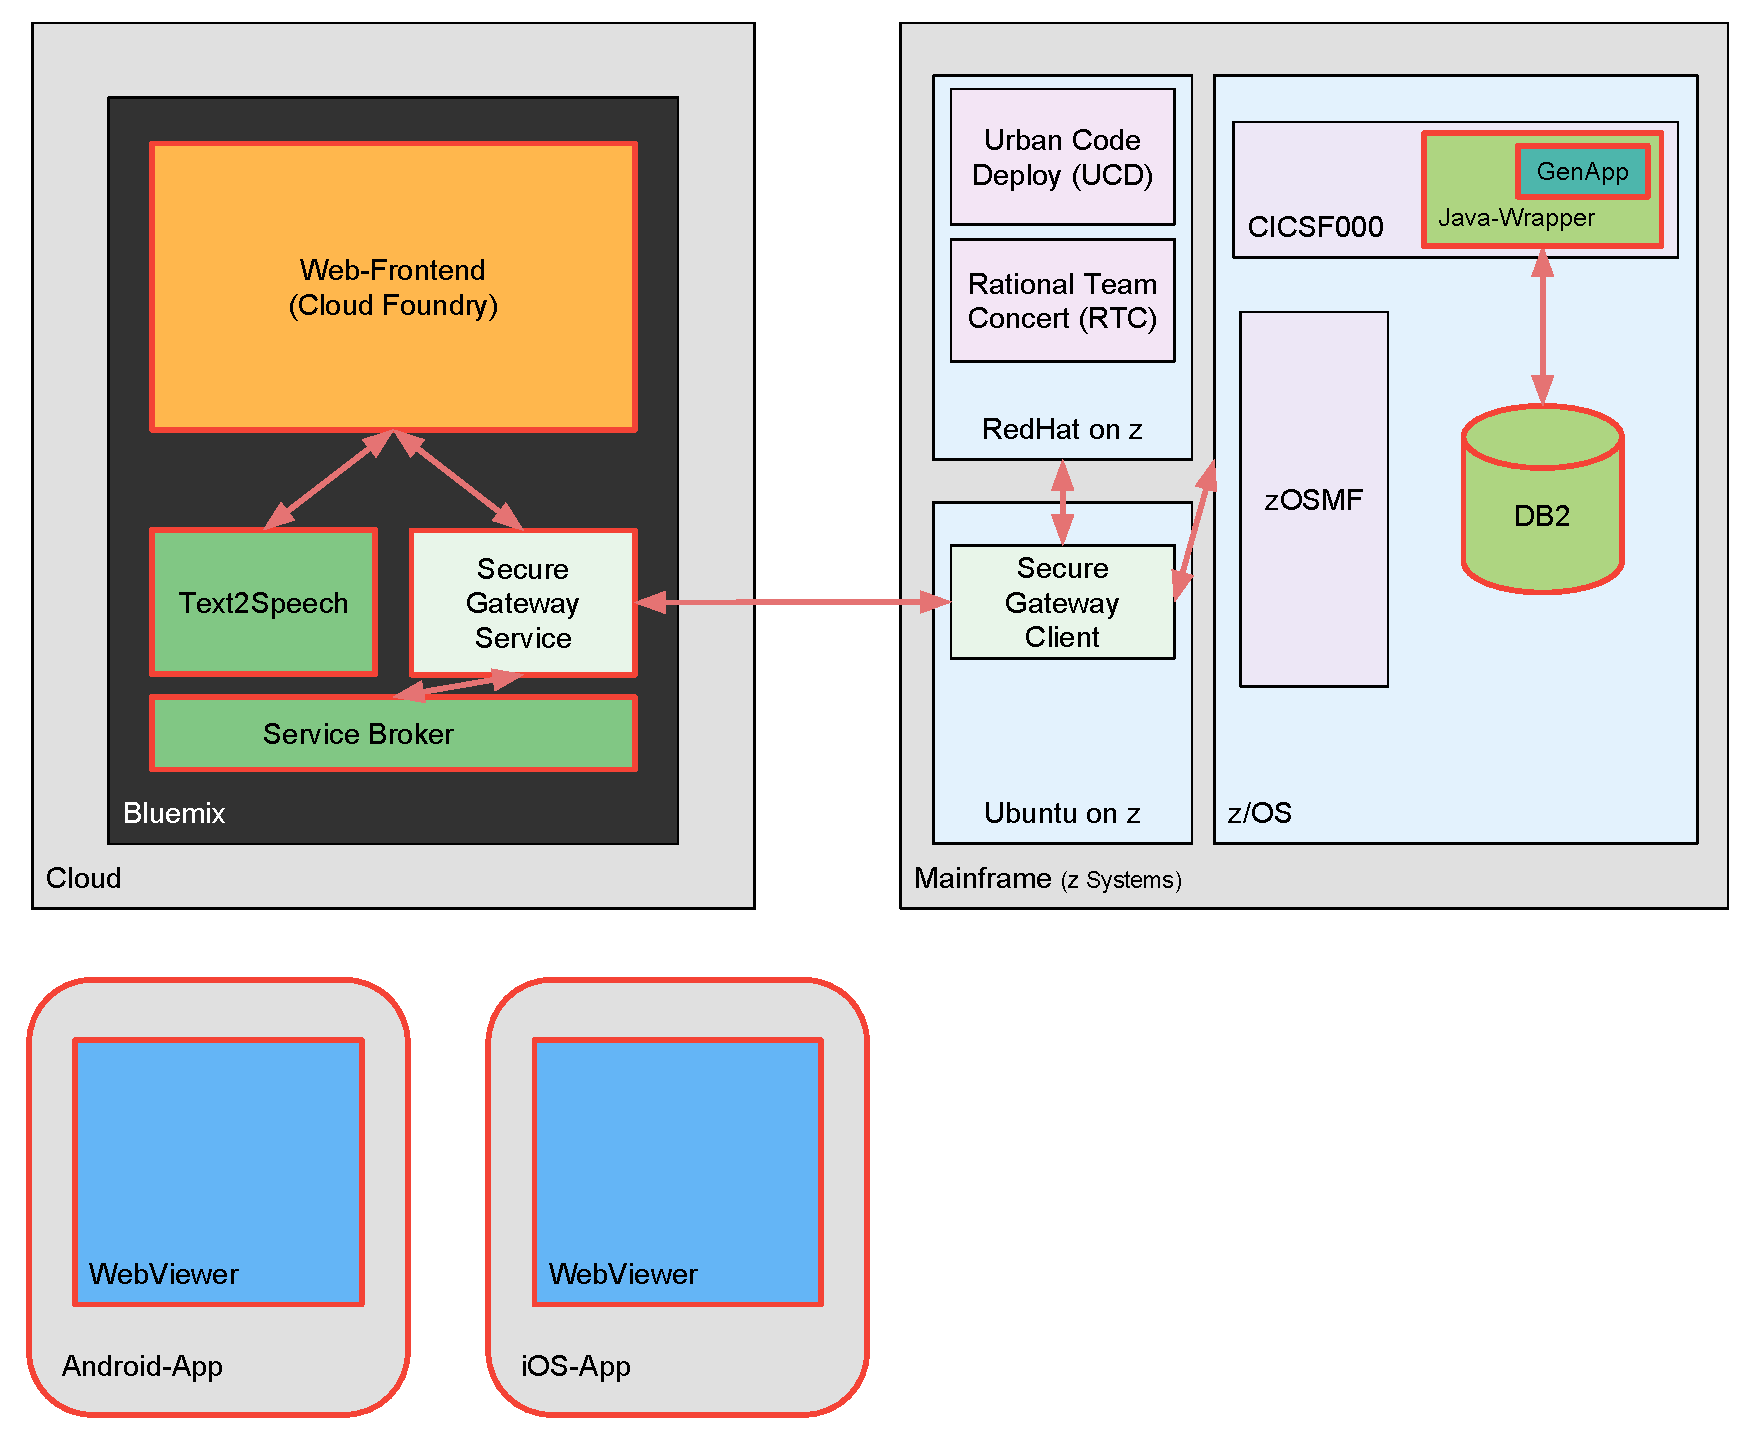
\includegraphics[scale=0.5]{images/kapitel_4/architektur_gesamtuebersicht.pdf}
  \caption{Übersicht über die Zielimplementierung}
  \label{fig:architektur_gesamtuebersicht}
\end{figure}

\subsection{COBOL-Anwendung}
Für den Start der prototypischen Implementierung der Hybrid-Cloud-Architektur wird eine vorhandene Applikation benötigt,
welche im Unternehmen eingesetzt wird oder produktiv ist.

Viele Unternehmen haben ihn ihrem Repertoire von alten aber dennoch eingesetzten Programmen durchaus COBOL-Anwendungen
in CICS-Regionen am laufen. Dies soll zum Anlass genommen werden, eine solche Anwendung ohne Anpassungen am Quellcode
für die Cloud bereit zu stellen.

In diesem Beispiel handelt es sich um die generische Applikation \path{GenApp}, für die die Oberfläche in Abbildung
\ref{fig:ibmad_map} auf Seite \pageref{fig:ibmad_map} zu sehen ist.

\begin{figure}[h]
  \centering
    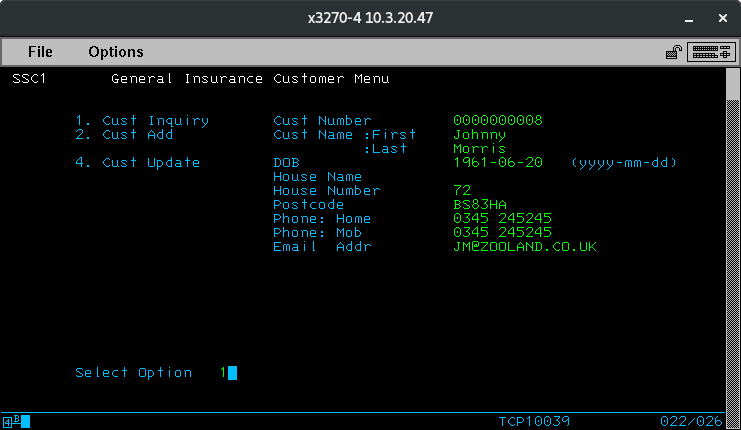
\includegraphics[scale=0.5]{images/kapitel_4/ibmad_map.png}
  \caption{Grafische Benutzeroberfläche der COBOL-Anwendung}
  \label{fig:ibmad_map}
\end{figure}

Der Transaktionsname der GenApp lautet \path{SSC1}. Durch einen Terminalaufruf des Namens in der CICS-Region wird die
Anwendung gestartet. Beim Start der Anwendung wird zuallererst die Oberfläche, die \path{BMS Map}, geladen und dem Nutzer
angezeigt.

Diese COBOL-Anwendung kann Daten aus einer Datenbank auslesen, diese bearbeiten oder neue Datensätze anlegen. Bei der
verbundenen Datenbank handelt es sich um eine DB2.

Durch eintragen einer Nummer hinter \path{Cust Number} und anschließendem ausführen der Funktion \path{Cust Inquiry}
werden die hinterlegten Informationen angezeigt. In der Abbildung sind das die Informationen des Kunden mit der Nummer
\path{8}.

Wenn Informationen überschrieben werden, können diese mit der Funktion \path{Cust Update} in der Datenbankt persistiert
werden.

Über den Parameter \path{Cust Add} und dem Hinzufügen von Informationen hinter den einzelnen Kategorien wird ein neuer
Kunde hinzugefügt.

Die Auswahl der Funktion, also \path{Cust Inquiry}, \path{ Cust Update} und \path{Cust Add}, erfolgt durch die Eingabe der
entsprechenden Zahl hinter \path{Select Option}.

Die drei Funktionen zum Verwalten der Daten, sollen dem Web-Frontend in der Cloud bereitgestellt werden. Da die genaue
Funktionsweise der Applikation jedoch nicht bekannt ist, müssen die internen Aufrufe und Übergabeparameter analysiert
werden.

\subsubsection{Analysieren der Anwendung}
Für die Analyse der COBOL-Anwendung wird das Programm \textit{IBM Application Discovery} (kurz IAD) genutzt. Eine
Übersicht der Anwendung ist in Abbildung \ref{fig:ibmad_uebersicht} auf Seite \pageref{fig:ibmad_uebersicht} zu sehen.

\begin{figure}[h]
  \centering
    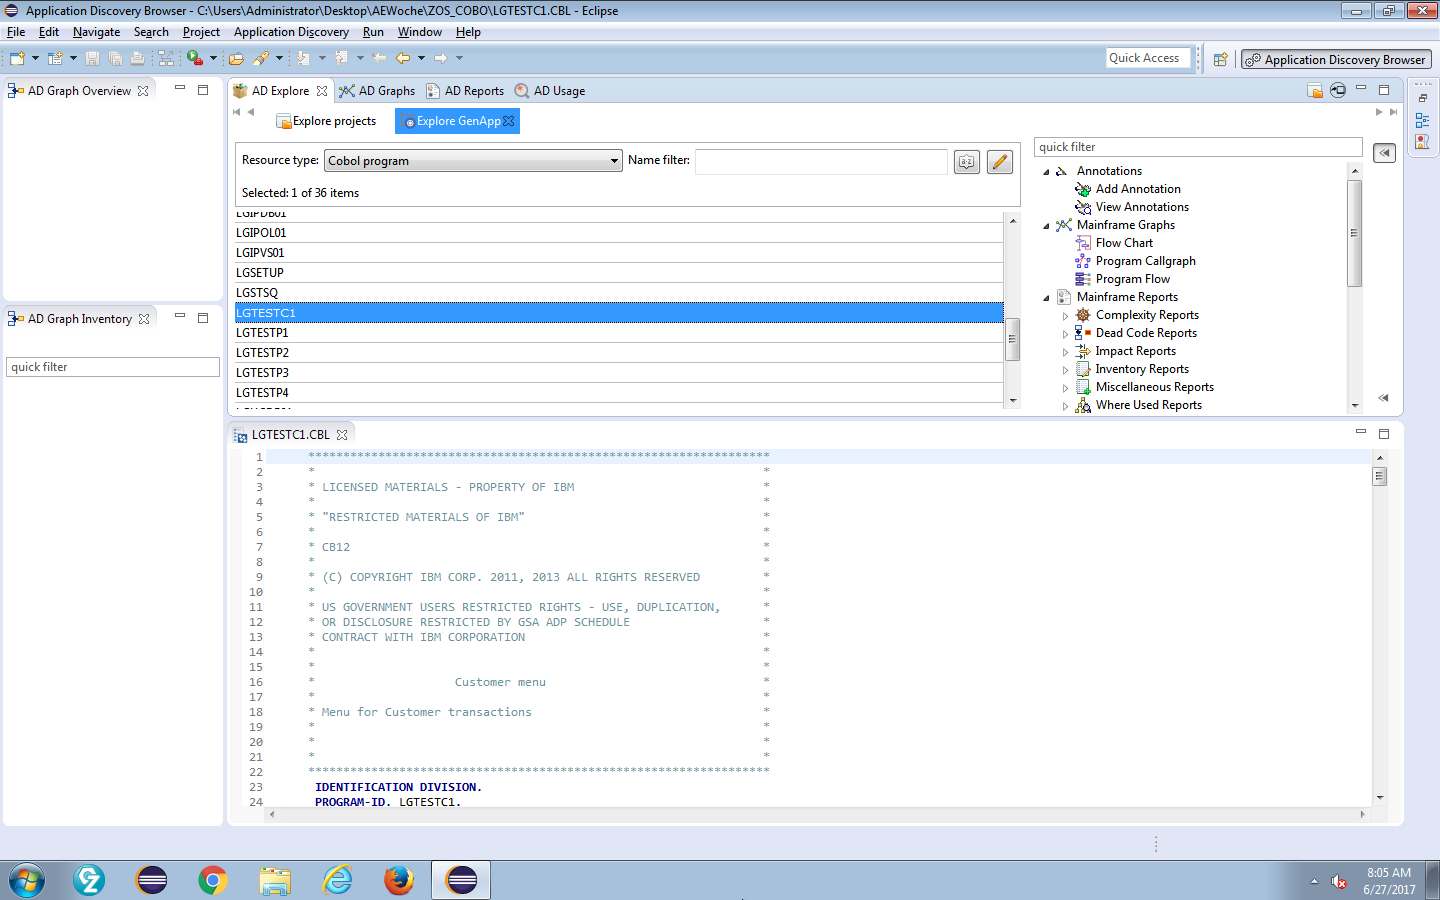
\includegraphics[scale=0.27]{images/kapitel_4/ibmad_uebersicht.png}
  \caption{Übersicht über IBM Application Discovery}
  \label{fig:ibmad_uebersicht}
\end{figure}

Dort ist zu sehen, dass \path{LGTESTC1} ausgewählt und der Quellcode ersichtlich ist. Bei diesem Teilprogramm der
Anwendung handelt es sich um das \textit{Mainprogramm} der Anwendung, welches beim Starten zuallererst aufgerufen wird.

Diese Tatsache kann durch das Vergleichen des \path{Callgraph} der Anwendung herausgefunden werden. In der Abbildung
\ref{fig:ibmad_callgraph} auf Seite \pageref{fig:ibmad_callgraph} ist zu sehen, dass der Terminalaufruf \path{SSC1}, welcher
die Anwendung startet, das Programm \path{LGTESTC1} ausführt.

Dieses Programm initialisiert dann die grafische Oberfläche der Anwendung, die SSMAP.

\begin{figure}[h]
  \centering
    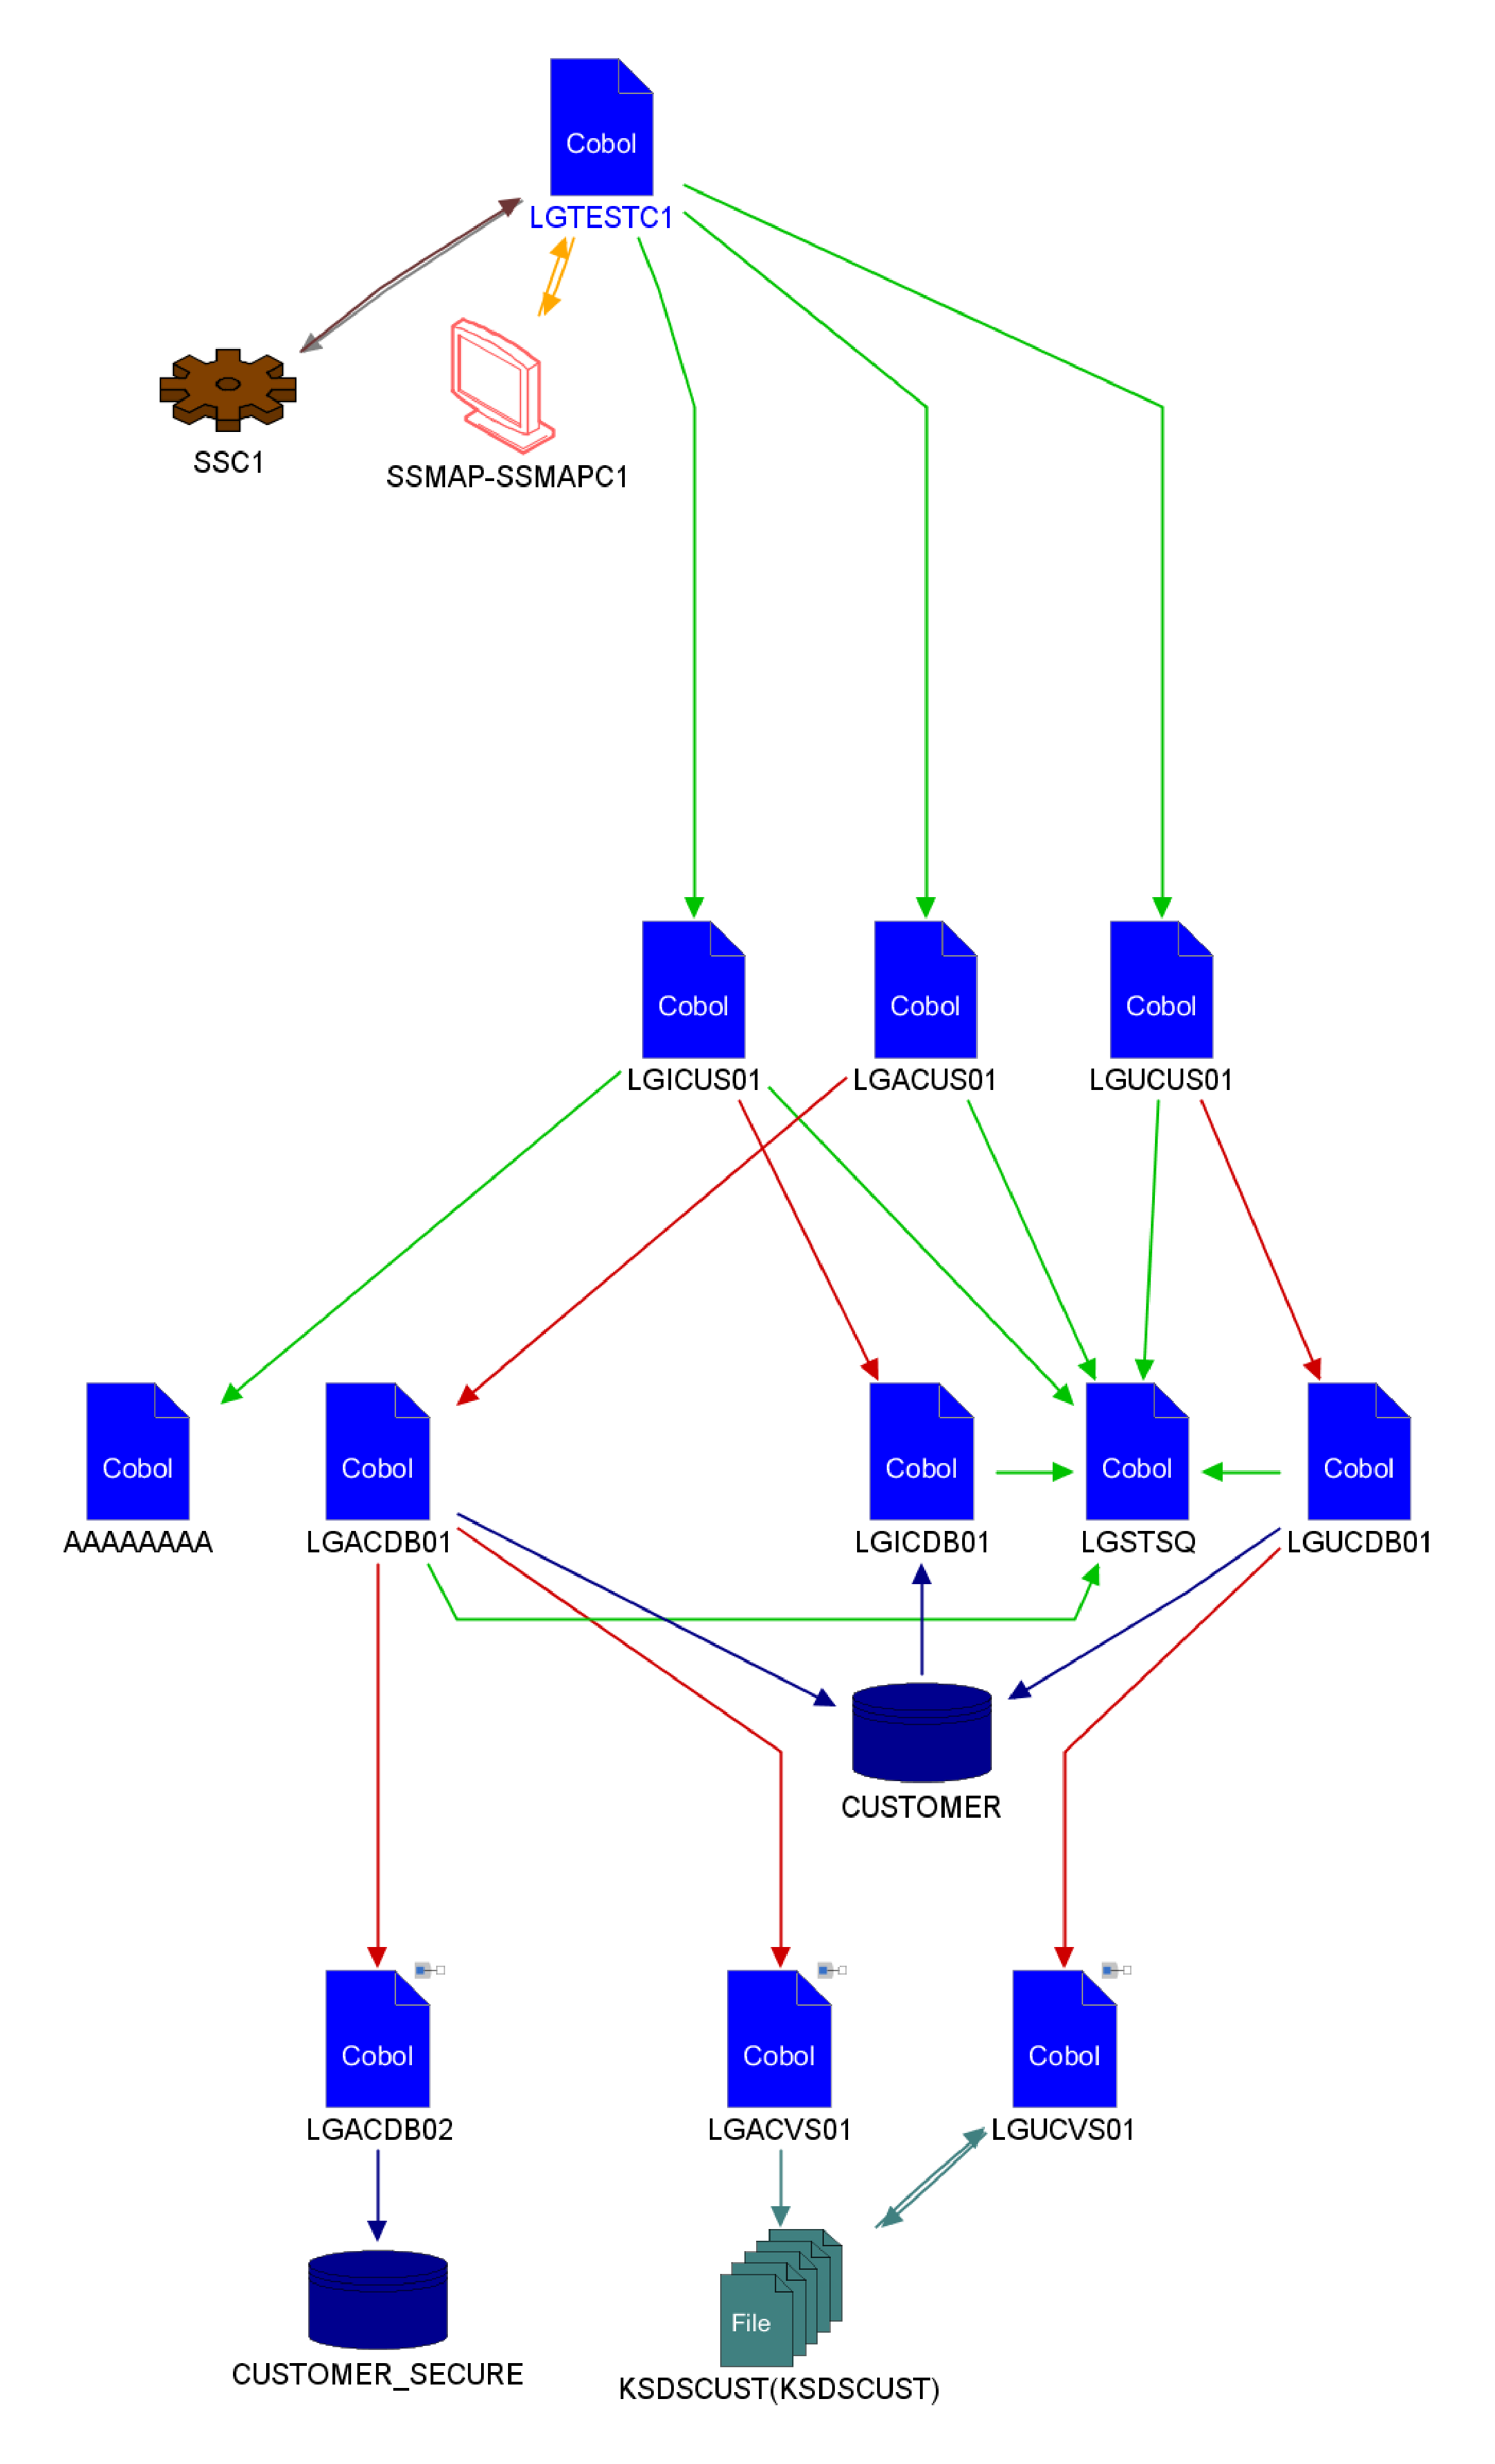
\includegraphics[scale=0.25]{images/kapitel_4/ibmad_callgraph.pdf}
  \caption{Der Callgraph der GenApp}
  \label{fig:ibmad_callgraph}
\end{figure}

Es existiert eine dauerhafte Verbindung zwischen der GUI und dem Hauptprogramm. So können Benutzereingaben direkt in der
Anwendung registriert und abgearbeitet werden.

Dieser Callgraph der Anwendung kann über die Funktion \path{Program Callgraph} im Bereich \path{Mainframe Graphs} im
rechten Kasten ausgewählt und angeschaut werden.

Im Callgraph ist darüber hinaus ebenfalls zu sehen, dass je nach Auswahl des Benutzers im Hauptprogramm das Programm
\path{LGICUS01}, \path{LGACUS01} oder \path{LGUCUS01} gestartet wird. Dies lässt vermuten, dass es eine Switch-Verzweigung
gibt, welche durch den Benutzer ausgelöst wird.

Mit der Ansicht des kompletten Flow-Diagramms \ref{anhang:flowchart} auf Seite \pageref{anhang:flowchart} lässt sich die
genaue Verzweigung extrahieren. Siehe dazu Abbildung \ref{fig:ibmad_flowchartSwitch} auf Seite
\pageref{fig:ibmad_flowchartSwitch}.

\begin{figure}[h]
  \centering
    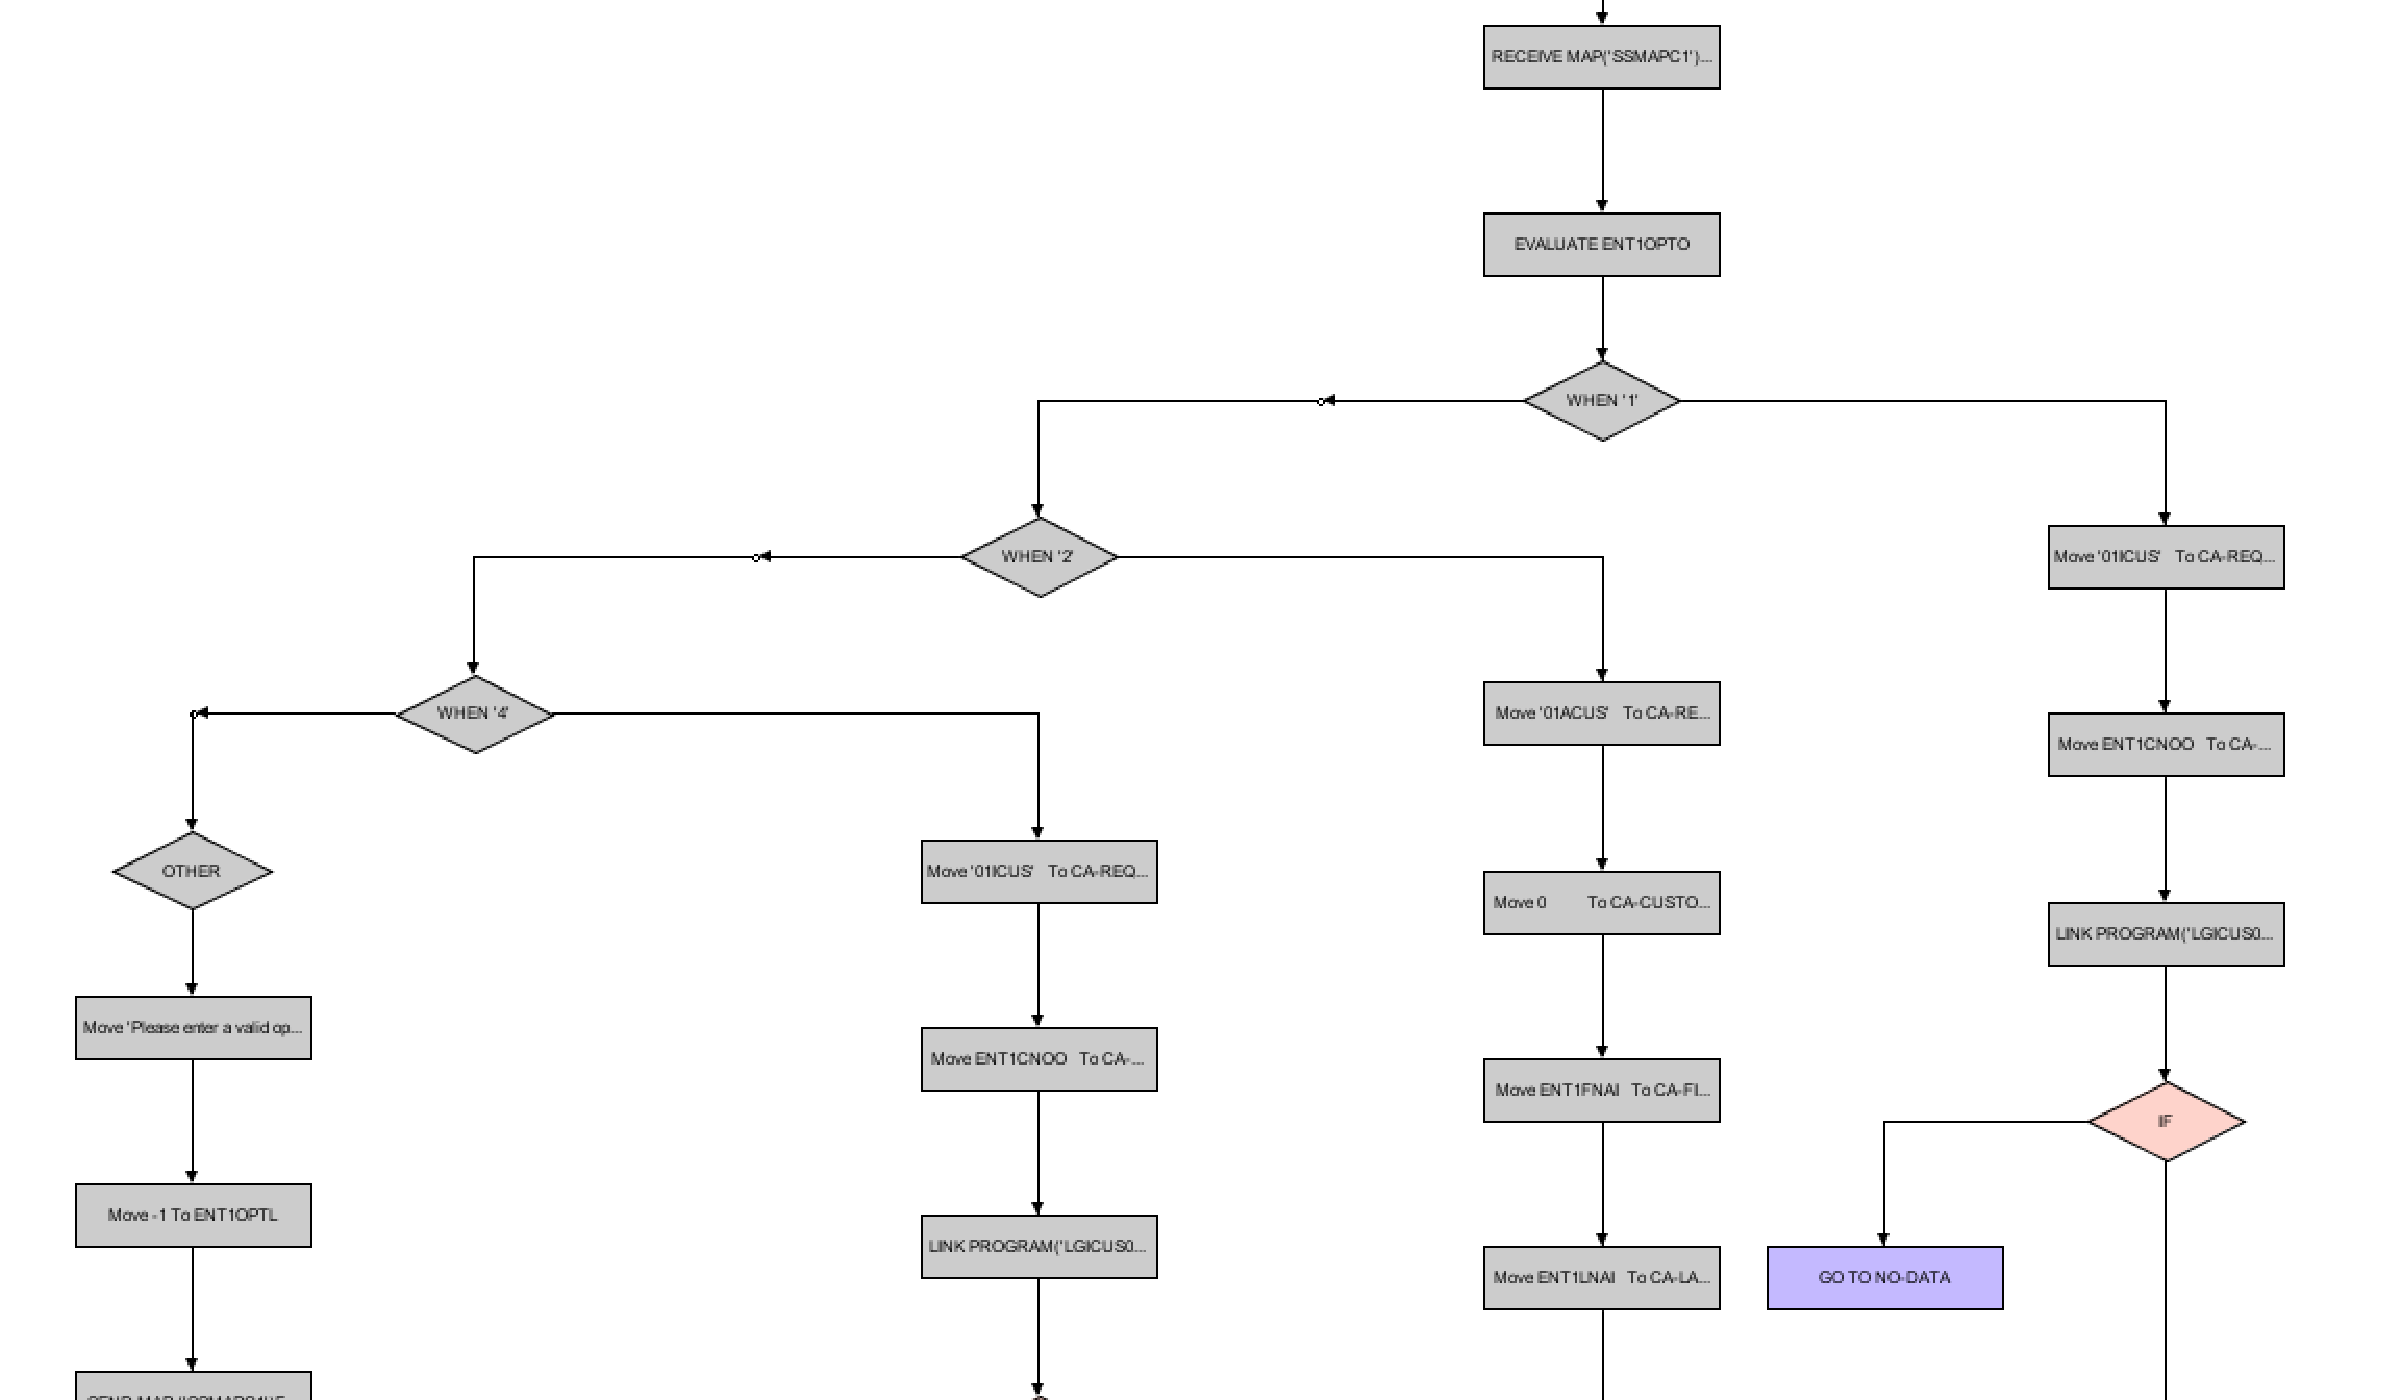
\includegraphics[scale=0.35]{images/kapitel_4/ibmad_flowchartSwitch.pdf}
  \caption{Die Switch-Verzweigung der GenApp}
  \label{fig:ibmad_flowchartSwitch}
\end{figure}

Das Flow-Diagram lässt sich in IBM Application Discovery mit der Schaltfläche \path{Flow Chart} anzeigen und es wird ein
Diagramm wie in Abbildung \ref{fig:ibmad_graph} auf Seite \pageref{fig:ibmad_graph} sichtbar.

In diese kann dann nach belieben rein- und rausgezoomt werden. Auch lassen sich Bilder extrahieren und Programmteile
genauer untersuchen.

\begin{figure}[h]
  \centering
    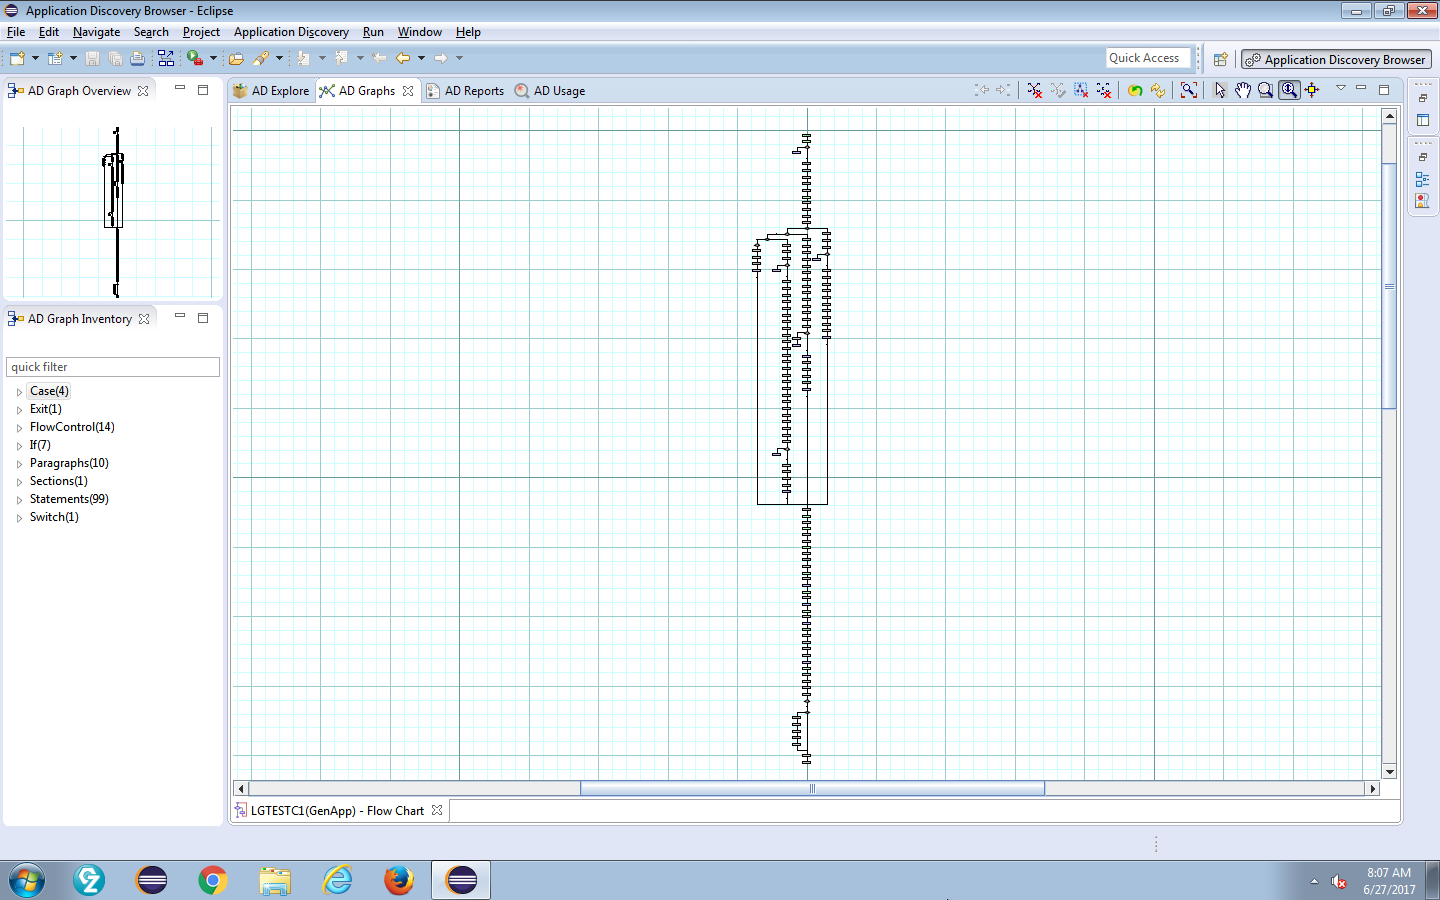
\includegraphics[scale=0.28]{images/kapitel_4/ibmad_graph.png}
  \caption{Anzeigen des Flow Charts}
  \label{fig:ibmad_graph}
\end{figure}

Aus dem Flow-Chart und der daraus extrahierten Switch-Verzweigung lässt sich eine wichtige Kenntnis ableiten. Das
Hauptprogramm startet je nach Auswahl des Benutzers eine von drei unterschiedlichen Programmen. Diese Information kann
nun für die Definition der Schnittstellen genutzt werden.

\subsubsection{Definieren der Schnittstellen}
Da die Anwendung nun analysiert ist, können die verwendeten Schnittstellen der Anwendung ausgewählt und dokumentiert
werden. Bei den Schnittstellen handelt es sich lediglich um die einzelnen Aufrufe, welche bei der Switch-Verzweigung
in LGTESTC1 aufgerufen werden. Siehe dazu \ref{fig:ibmad_flowchartSwitch} auf Seite \pageref{fig:ibmad_flowchartSwitch}.

Damit der Java-Wrapper mit der COBOL-Anwendung genutzt werden kann muss dieser die Programmteile \path{LGICUS01},
\path{LGACUS01} und \path{LGUCUS01} starten können. Diese sind für die Verarbeitung der Daten zuständig.

Dabei ist \path{LGACUS01} für das Hinzufügen eines neuen Customers zuständig. Der Java-Wrapper muss dem Programm die
Informationen wie \textit{Vorname}, \textit{Nachname}, \textit{Wohnort}, \textit{Straßenname} und \textit{Telefonnummer}
übergeben.

Das Teilprogramm \path{LGUCUS01} kann einen Eintrag eines Customers aktualisieren. Dazu werden die neuen Werte als
Parameter übergeben. Dabei handelt es sich um die Selben wie bei LGACUS01.

Im letzten Programm, \path{LGICUS01}, werden Informationen des Customers zurückgegeben. Dazu werden keine Parameter zum
Aufruf benötigt. Lediglich werden Daten zurück an den Java-Wrapper gegeben.

Die Kommunikation zwischen Java-Wrapper und COBOL-Anwendung wird mittels der WOLA-Schnittstelle gewährleistet.

Diese Informationen können dazu genutzt werden, um den Java-Wrapper zu bauen, damit die COBOL-Anwendung für die Cloud
bereitgestellt werden kann.

\subsection{CICS Region erstellen}
Da nun die COBOL-Anwendung analysiert ist, kann eine CICS-Region erstellt werden, welche sowohl die COBOL-Anwendung
als auch den späteren Java-Wrapper beinhalten wird.

Dazu wird der instanziierte \path{Service Broker zOSMF} geöffnet und dann der Tab \path{CICS} ausgewählt. Nun werden alle
schon eingerichteten CICS-Regionen angezeigt.

Um eine neue Region zu erstellen, wird auf den Button \path{ADD CICS} geklickt, worauf sich ein Fenster öffnet, in dem
Informationen eingegeben werden müssen. Siehe dazu Abbildung \ref{fig:image_cicsErstellen} auf Seite
\pageref{fig:image_cicsErstellen}.

\begin{figure}[h]
  \centering
    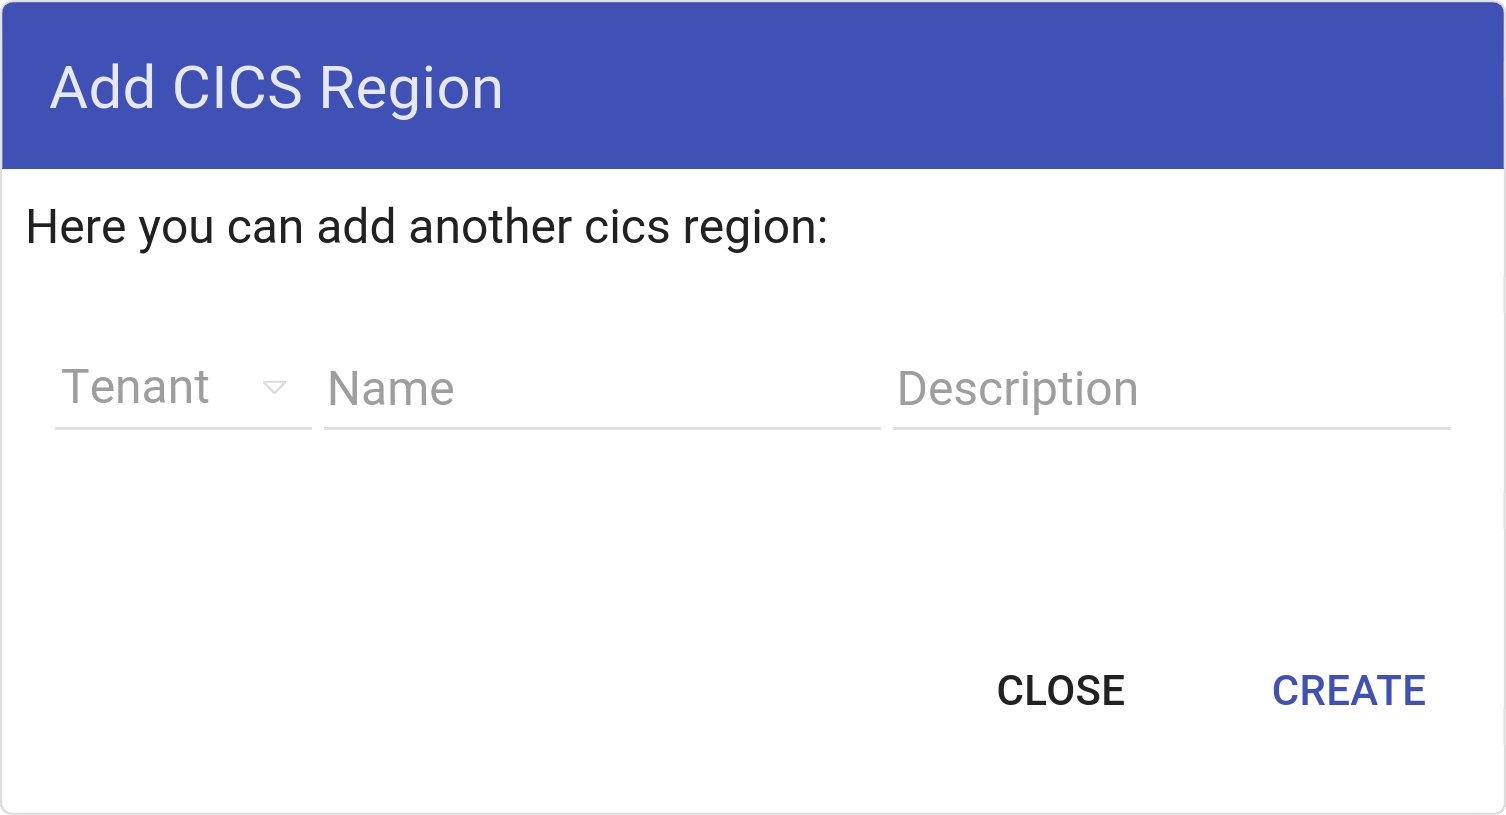
\includegraphics[scale=0.2]{images/kapitel_4/image_cicsErstellen.png}
  \caption{Erstellen einer CICS Region}
  \label{fig:image_cicsErstellen}
\end{figure}

Nach der Auswahl eines Tenanten (Standort), der Eingabe eines Namens und einer Beschreibung kann auf \path{CREATE} geklickt
werden, worauf die neue CICS-Region eingerichtet wird. Dieser Vorgang dauert ein paar Sekunden.

Im Anschluss wird die neue CICS-Region in der Übersicht angezeigt. Sie kann nun ausgewählt werden, um weitere Informationen
anzuzeigen. Insbesondere die Information über den \path{Port} spielt für die weitere Vorgehensweise eine wichtige Rolle.

\subsection{Verbindung aufbauen}
Da nun eine neue CICS-Region erstellt wurde, muss im Secure Gateway Service in Bluemix ein Eintrag für diese hinzugefügt
werden. Dies ermöglicht die Kommunikation mit der Region via URL und Port.

Dazu wird der Secure Gateway Service in Bluemix geöffnet und der eingerichtete Client angeklickt. Damit öffnet sich die
Übersicht über alle registrierten \path{Ziele}.

Über den großen grünen Knopf kann ein neues Ziel hinzugefügt werden. Dabei wird zuallererst nach dem Standort des Ziels
gefragt. Da sich die CICS-Region auf dem Mainframe befindet, wird hier \path{Lokal} ausgewählt.

Mit einem Klick auf \path{Weiter} wird nach dem Hostname und dem Port gefragt. Der Hostname ist die IP-Adresse des z/OS-Systems
(hier im Beispiel die \path{10.3.20.47}) und der Port ist der der neu erstellten CICS-Region. Hier im Beispiel also die
\path{54300}. Im Anschluss kann auf \path{Weiter} geklicken werden.

Nun können Zertifikate für die Autorisierung hochgeladen und die Art des Protokolls definiert werden. Hier im Beispiel
werden keine Zertifikate genutzt, und das Protokoll ist \path{TCP}, da dieses Protokoll auch für die Kommunikation zwischen
Ubuntu- und z/OS-System genutzt wird. Mit einem Klick auf \path{Weiter} wird dies bestätigt.

Im Folgenden kann die Authentifizierung ausgewählt werden. Da nun erstmal keine genutzt wird, kann die Auswahl bei
\path{None} gelassen und mittels \path{Weiter} gespeichert werden.

Da die Verbindung nicht eingeschränkt werden soll, kann das nächste Fenster einfach mit \path{Weiter} gespeichert werden,
worauf die Eingabe eines Namens für das Ziel folgt.

In diesem wird als Name \path{REST-Interface} genutzt, da in dieser CICS-Region sowohl die COBOL-Anwendung als auch das
REST-Interface laufen wird. Nach der Eingabe kann das Ziel gespeichert werden und es wird direkt in der Übersicht angezeigt.

Mit einem Klick auf das Zahnrad des jeweiligen Ziels öffnet sich ein Fenster mit verschiedenen Informationen zu diesem.
Dabei ist der Eintrag \path{Cloud-Host: Port} wichtig, da dieser die URL für die CICS-Region anzeigt, die im Web-Frontend
genutzt wird um die REST-Schnittstelle anzusprechen.

\subsection{Toolchain konfigurieren}
In Kapitel \ref{subsec:einrichten_der_toolchain} auf Seite \pageref{subsec:einrichten_der_toolchain} wurde die Toolchain
zum Bauen des Artefaktes aus dem Quellcode schon grundsätzlich eingerichtet. Da nun eine CICS-Region für das Backend
eingerichtet wurde und die Verbindung zwischen Bluemix und CICS-Region auf dem Mainframe hergestellt wird, kann nun auch
der Buildprozess darauf angepasst werden.

Dazu wird die Toolchain in Bluemix geöffnet und im Dashbaord dann die Build Pipeline ausgewählt. In dieser sind zwei Stages
vorkonfiguriert. Die \path{BUILD}-Stage baut immer nach einem \textit{push} in das Git-Repository ein Artefakt aus dem
Quelltext. Dieses Artefakt gibt sie weiter an die \path{DEPLOY}-Stage. Diese kann das Artefakt auf einem System
installieren. In diesem Fall muss diese angepasst werden.

Über das Zahnrad-Symbol am rechten oberen Rand der \path{BUILD}-Stage wird die Konfiguration geöffnet. In dem sich
öffnenden Fenster wird unter \path{Jobs} über den Button \path{Job hinzufuegen} ein neuer hinzugefügt. Der Typ dabei ist
\path{Build}. Dieser erhält als Namen zum Beispiel \path{Deploy on CICS}. Als Buildtyp wird \path{Shell-Script} ausgewählt
und das Build-Script kann in Listing \ref{Build-Script für CICS-Region} auf Seite \pageref{Build-Script für CICS-Region}
eingesehen werden.

\begin{lstlisting}[language=bash, caption=Build-Script für CICS-Region, label=Build-Script für CICS-Region]
    #!/bin/bash
    sudo apt-get update && sudo apt-get install lftp
    lftp -u username,password -e 'mirror ./GenAppService.war /var/cicsts/CICSF000/workdir/DFHWLP/wlp/usr/servers/defaultServer/dropins/' secureGatewayURL:PORT
\end{lstlisting}

Dabei sind die Parameter \path{username} und \path{password} die, eines Benutzers auf der z/OS Maschine. Dabei können es
die Selben der zOSMF-Schnittstelle sein. Der Benutzer muss lediglich Schreibrechte im \path{dropins}-Verzeichnis haben.

Der Parameter \path{secureGatewayURL} mit zugehörigem \path{PORT} ist in Bluemix im Secure Gateway Service zu finden,
nachdem die CICS-Region damit verbunden wurde.

Durch dieses Shell-Script, wird in einer Virtuellen Umgebung in der Toolchain das Programm
\path{LFTP}\footnote{https://lftp.yar.ru} installiert. Anschließend wird mit Hilfe des Programms das Artefakt aus dem
vorhergehenden Build-Step auf die CICS-Region kopiert und gegebenenfalls überschrieben.

Da die CICS-Region einen WebSphere Liberty Server enthält und dieser Application Server alle \path{.war}-Files im
\path{dropins}-Verzeichnis automatisch einbindet, kann die \path{GenAppService.war}-Datei einfach dort abgelegt werden.
Nach wenigen Sekunden importiert der Server die Datei dann automatisch und stellt sie dem Benutzer zur Verfügung.

Nun wird nach jedem \textit{push} in das Git-Repository automatisch der Build and Deploy vorgang (Build Pipeline) gestartet
und die neueste Version der Anwendung auf der verbundenen CICS-Region installiert.

\subsection{Runtime hinzufügen}
\label{subsec:runtime_hinzufügen}
Da nun die Verbindung zwischen Cloud-Infrastruktur und CICS-Region hergestellt ist, kann im nächsten Schritt die Runtime
für das Web-Frontend instanziiert und eingerichtet werden.

Um in Bluemix eine Runtime für NodeJS-Applikationen zur Verfügung zu stellen, gibt es zwei Möglichkeiten.

\subsubsection{Einrichtung mittels Bluemix Dashbaord}
\label{subsubsection:bluemixDashbaord}
Die Einrichtung einer Runtime für NodeJS mittels Bluemix Dashboard startet mit einem Aufruf des \path{Katalogs} in Bluemix.
In diesem gibt es unter der Kategorie \path{Apps} und \path{Cloud Foundry-Anwendungen} den Eintrag \path{SDK for NodeJS}.

Ein Klick auf den Eintrag öffnet die Übersicht des Services. Der Name definiert den Namen der Runtime wie sie unter
Bluemix aufgelistet wird. Der Hostname definiert die URL, über die die Anwendung aufrufbar ist. Sie folgt dabei dem Schema
\path{https://hostname.mybluemix.net}.

Nach dem Klick auf \path{Erstellen} wird die Runtime eingerichtet und vorbereitet. Dieser Schritt dauert je nach
Gesamtauslastung von Bluemix wenige Sekunden.

Im Anschluss ist die Runtime im Dashboard von Bluemix zu finden und einsatzbereit. Der Aufruf der definierten Domain
im Webbrowser öffnet eine Standardseite mit Informationen zur Runtime.

\subsubsection{Einrichtung mittels Cloud Foundry CLI}
Eine Alternative zur Einrichtung der Runtime via Dashboard ist die Einrichtung via Cloud Foundry CLI. Dazu wird die CF CLI
mittels \path{login} mit der aktuellen Organisation und dem Bereich verbunden und im Anschluss mittels \path{create-service}
eine SDK for NodeJS eingerichtet.

\begin{lstlisting}[language=bash, caption=Provisionieren des SDK for NodeJS Services, label=Provisionieren des SDK for NodeJS Services]
   $ cf create-service sdk_for_nodejs standard appName
\end{lstlisting}

Dabei ist \path{sdk_for_nodejs} der Name des Service, der instanziiert werden soll. Der Parameter \path{standard} gibt an,
dass der einzig verfügbare Plan genutzt werden soll. Als letztes gibt \path{appName} den Hostnamen, welcher verwendet
werden soll, an.

Die Einrichtung sollte innerhalb weniger Sekunden abgeschlossen sein, und die Runtime wird im Bluemix Dashboard angezeigt.
Alle aktiven Runtimes mit Name und Hostname können über den Befehl \path{apps} aufgelistet werden.

\begin{lstlisting}[language=bash, caption=Auflisten aller Applikationen, label=Auflisten aller Applikationen]
   $ cf apps
\end{lstlisting}

Nun kann die Anwendung über den definierten \path{appName} in einem Webbrowser aufgerufen werden, und es erscheint eine
Standartseite mit Informationen zur Runtime.

\subsection{Text2Speech-Service hinzufügen}
Da nun die Runtime für das Web-Frontend erstellt und eingerichtet ist, kann der zusätzlich genutzte Service \path{Text2Speech}
instanziiert werden. Dieser wandelt geschriebenen Text in eine Audio-Datei um, die von modernen Webbrowsern abgespielt
werden kann.

Da dies, genau wie die Runtime SKD for NodeJS, auch ein Service ist, gibt es auch hier beide Möglichkeiten der Einrichtung,
entweder über das Bluemix Dashboard oder über das Cloud Foundry CLI. Der einfachheithalber wird hier nur der Weg mittels
CLI aufgezeigt. Die Einrichtung mittels Bluemix Dashboard erfolgt analog zu Kapitel \ref{subsubsection:bluemixDashbaord}
auf Seite \pageref{subsubsection:bluemixDashbaord}.

Mit \path{create-service} wird der Service dem Bluemix Account hinzugefügt und steht ab dann zur Verfügung.

\begin{lstlisting}[language=bash, caption=Provisionieren des Text2Speech Services, label=Provisionieren des Text2Speech Services]
   $ cf create-service text_to_speech standard serviceName
\end{lstlisting}

Mit dem Befehl \path{services} können alle instanziierten Services in der Organisation und dem Bereich angezeigt werden.

\begin{lstlisting}[language=bash, caption=Auflisten aller instanziieren Services, label=Auflisten aller instantiieren Services]
   $ cf services
\end{lstlisting}

\subsection{Runtime verbinden}
Damit die SDK for NodeJS Runtime und der Service Text2Speech über die \path{VCAP} Variablen kommunizieren können, müssen
die App und der Service verbunden werden. Um diesen Schritt durchzuführen, gibt es zwei Möglichkeiten.

\subsubsection{Binden über Bluemix Dashboard}
Um die Runtime und den Service über das Bluemix Dasboard zu verbinden, muss die Übersichtsseite der SDK for NodeJS Runtime
geöffnet werden. Auf dieser Übersichtsseite gibt es den Tab \path{Verbindungen}. In diesem werde alle Verbindungen zwischen
Runtime und Services angezeigt. Zur Zeit existieren noch keine.

Mit einem Klick auf \path{Vorhandenen verbinden} kann der schon erstellte Text2Speech Service verbunden werden. In der sich
öffnenden Seite wird dieser dazu einfach ausgewählt und mittels \path{Verbindung herstellen} gespeichert.

Die Frage, ob die Runtime neu gestaged (neugestartet und verbunden) werden darf, muss mit \textbf{Ja} bestätigt werden.
Die Runtime steht ab dann für wenige Sekunden nicht zu Verfügung.

Anschließend erscheint der Text2Speech Service auf der Übersichtsseite der Runtime im Tab \path{Verbindungen}.

\subsubsection{Binden über Cloud Foundry CLI}
Alternativ kann die Verbindung über die Cloud Foundry CLI durchgeführt werden. Dazu wird die Funktion \path{bind-service}
nach einem vorangegangenen \path{login} genutzt.

\begin{lstlisting}[language=bash, caption=Binden der Runtime mit dem Service, label=Binden der Runtime mit dem Service]
   $ cf bind-service appName serviceName
\end{lstlisting}

Dabei wird als \path{appName} der vergebene Name der NodeJS-Runtime angegeben. Als \path{serviceName} der Name, der an den
Text2Speech Service vergeben wurde.

Anschließend muss die Runtime mittels \path{restart} neugestartet werden.

\begin{lstlisting}[language=bash, caption=Neustarten der Runtime, label=Neustarten der Runtime]
   $ cf restart appName
\end{lstlisting}

Dabei wird wieder als \path{appName} der Name der NodeJS-Runtime angegeben.

Die erfolgreiche Verbindung der Runtime und des Service ist in der Übersichtsseite der Runtime im Bluemix Dashboard im
Tab \path{Verbindungen} sichtbar.

\subsection{Erstellen des Backends}
Damit das Frontend die Daten aus der Datenbank visualisieren kann, müssen diese aus dem Backend abgerufen werden. Dies kann
auf zwei Arten geschehen.

In der ersten Möglichkeit ruft das Frontend die Daten durch den Java-Wrapper ab, der wiederum die Daten durch die
COBOL-Anwendung von der Datenbank erhält.

Alternativ kann das Frontend auch einen REST-Service der DB2 abrufen, welcher aufgrund eines hinterlegten SQL-Befehls
Daten zurückgeben kann.

Ein Auszug des Datenbankaufbaus ist in Anhang \ref{anhang:datenbankschema} auf Seite \pageref{anhang:datenbankschema}
zu sehen. Da die GenApp schon verschiedene Daten aus der Datenbank zurückgeben kann, wird der DB2 Service nur für die
Daten genutzt, welche nicht durch die GenApp erfasst werden. Somit können beide Varianten nebeneinander koexistieren, ohne
sich zu überlagern.

Ein weiterer Grund ist, dass die COBOL-Anwendung in ihrer Funktionalität nicht erweitert werden soll.

\subsubsection{DB2 REST Services}
Da die COBOL-Anwendung lediglich die \textit{Kundeninformationen} und die \textit{Policies} aus der Datenbank lesen kann,
und keine Information darüber hat, welcher Kunde welche Policy besitzt, wird ein DB2 Rest Service eingerichtet, der diese
Information auflösen kann.

Um einen DB2 REST Service anzulegen, wird ein Package in der DB2 Instanz eingerichtet. Dieses Package enthält eine
SQL-Abfrage und wird im \path{SYSIBM.DSNSERVICE} Katalog abgelegt.

Ein authentifizierter Benutzer kann sich alle für ihn sichtbaren Services anschauen, diese ausführen und einen neuen
einrichten.

Weitere Informationen über den Service sind im IBM Knowledge
Center\footnote{https://www.ibm.com/support/knowledgecenter/SSEPEK\_11.0.0/restserv/src/tpc\\/db2z\_restservices.html} zu
finden.

Da es sich bei der prototypischen Anwendung um eine Web-Anwendung handelt, welche direkt mit dem DB2 REST Service
kommunizieren wird, muss die DB2 Instanz CORS zulassen.

Dazu wird im z/OS-System, in welchem die DB2 Instanz läuft, in der Datei \path{/qibm/userdata/qwebqry/WQLIB85/conf/httpd.conf}
der Header für CORS - \\ \path{Access-Control-Allow-Origin} - gesetzt.

Für die Bearbeitung der Datei wird diese zum Beispiel mit \path{nano} geöffnet.

\begin{lstlisting}[language=bash, caption=Bearbeiten der Konfigurationsdatei, label=Bearbeiten der Konfigurationsdatei]
   $ nano /qibm/userdata/qwebqry/WQLIB85/conf/httpd.conf
\end{lstlisting}

Im Anschluss wird im \path{Location}-Tag der Header-Wert hinzugefügt.

\begin{lstlisting}[caption=Header für CORS setzen, label=Header für CORS setzen]
   $ Header set Access-Control-Allow-Origin "*"
\end{lstlisting}

Da nun mittels JavaScript-Requests der REST Service aufgerufen werden kann, kann dieser eingerichtet werden. Dazu wird
ein \path{POST}-Request an den DB2ServiceManager geschickt, welcher die Informationen für den Service beinhaltet.

Zum Ausführen des \path{POST}-Requests wird \path{Postman} genutzt. Dabei wird als URL die des DB2ServiceManager angegeben.

\begin{lstlisting}[language=bash, caption=DB2 REST Service erstellen, label=DB2 REST Service erstellen]
   POST https://<host>:<port>/services/DB2ServiceManager
\end{lstlisting}

Als \path{POST}-Parameter werden neben Typ und Name auch der SQL-Befehl übergeben, welcher ausgeführt werden soll, wenn der
Service aufgerufen wird.

\begin{lstlisting}[language=json, caption=Parameter zur Erstellung, label=Parameter zur Erstellung]
    {
        "requestType":  "createService",
        "sqlStmt":      "<sqlStatement>",
        "collectionID": "<serviceCollectionID>",
        "serviceName":  "<serviceName>",
        "description":  "<serviceDescription>"
    }
\end{lstlisting}

Dabei ist \path{requestType} der Typ der Anfrage. Dieser muss \path{createService} sein, da ein neuer Service in der
DB2 Instanz eingerichtet werden soll.

Bei \path{sqlStmt} handelt es sich um das SQL-Statement, welches bei einem Aufruf des Services ausgeführt werden soll.
Dabei gelten die Rechte des Nutzers, mit welchem der REST Service eingerichtet wurde.

Die \path{collectionID} ist der Benutzername für welchen der Service eingerichtet werden soll.

Der \path{serviceName} kann frei vergeben werden. Er wird beim Aufruf des Services genutzt, um ihn eindeutig zu
identifizieren und anzusprechen. In diesem Beispiel wird dafür \path{getPolicyByCustomer} genutzt.

Im Parameter \path{description} kann noch eine optinale Beschreibung des Services hinzugefügt werden.

Der Aufruf muss als eingeloggter Benutzer erfolgen. Dazu wird in Postman im Bereich \path{Authorization} der Type
\path{Basic Auth} ausgewählt und in die beiden Felder der Benutzername und das zugehörige Passwort eingetragen, für den
der Service eingerichtet werden soll. Der Benutzername muss der Selbe sein, welcher im POST-Parameter \path{collectionID}
verwendet wird.

Die Antwort des Servers nach dem Ausführen des Requests bestätigt die erfolgreiche Einrichtung des Services und zeigt die
\path{URL} an, welche zur Nutzung des Services genutzt wird.

\begin{lstlisting}[language=json, caption=Antwort des Servers, label=Antwort des Servers]
    {
     "StatusCode": 201,
     "StatusDescription": "DB2 Rest Service getPolicyByCustomer was created successfully.",
     "URL": "http://<host>:<port>/services/SYSIBMSERVICE/getPolicyByCustomer"
    }
\end{lstlisting}

Der HTTP-Statuscode mit \path{201} gibt an, dass der Service erfolgreich erstellt wurde.

Für die Anwendung ist die getPoliciesByCustomer-URL, \path{http://<host>:<port>/services/SUCI101/getPoliciesByCustomer},
erfolgreich eingerichtet worden.

\subsubsection{Secure Gateway Ziel}
Damit das Web-Frontend auf den erfolgreich eingerichteten DB2 REST Service zugreifen kann, um die Daten aus der Datenbank
auszulesen, muss nun ein weiteres Ziel für den Secure Gateway hinzugefügt werden.

Dies geschieht wie in Kapitel \ref{subsection:secureGateway} auf Seite \pageref{subsection:secureGateway} beschrieben.
Dabei ist der Name des Ziels nun \path{DB2 REST Service}. Die IP-Adresse und der Port sind die, welche nach erfolgreicher
Ausführung des \path{POST}-Request an den DB2ServiceManager zurückgegeben wurden. Siehe dazu Listing
\ref{Antwort des Servers} auf Seite \pageref{Antwort des Servers}.

\subsubsection{Java-Wrapper}
Damit das Web-Frontend Informationen aus der Datenbank über die schon analysierte COBOL-Anwendung abrufen kann, muss diese
mit einer Schnittstelle versehen werden. Diese Schnittstelle wird in Form eines Java REST-Interfaces zur Verfügung
gestellt, welches die Kommunikation zwischen Web-Frontend und COBOL-Anwendung übernimmt.

Damit der Java-Wrapper aus der Cloud über den Secure Gateway aufgerufen werden kann, muss der Application Server CORS
akzeptieren. Um CORS in WebSphere Liberty zu aktivieren muss der Header in der Konfiguration gesetzt werden.

Dazu wird in der jeweiligen \path{server.xml}-Datei im WebSphere-Verzeichnis der CICS-Anwendung der \path{cors}-Tag
eingefügt. Siehe dazu Listing \ref{Konfiguration von CORS} auf Seite \pageref{Konfiguration von CORS}.

\begin{lstlisting}[language=html, caption=Konfiguration von CORS, label=Konfiguration von CORS]
    <cors domain="*"
          allowedOrigins="*"
          allowedMethods="GET, DELETE, POST, OPTION"
          allowedHeaders="accept"
          allowCredentials="true"
          maxAge="3600" />
\end{lstlisting}

Durch diese Konfiguration kann jeder Client, symbolisiert durch \path{allowedOrigins="*"}, auf alle Entpunkte des
REST-Interfaces, \path{domain="*"}, zugreifen und das Interface nutzen.

Im Normalfall würde CORS bei \path{allowedOrigins="*"} nicht mit einem * konfiguriert werden, sondern
auf die wenigen Clients eingeschränkt, die wirklich Zugriff brauchen. Da bei der Entwicklung allerdings von
verschiedenen Testsystemen und produktiven Hosts zugegriffen wird, wird der Zugriff für die Entwicklungsdauer nicht
eingeschränkt.

Da nun CORS vom Server akzeptiert wird, kann das eigentliche Interface entwickelt werden. In Abbilung
\ref{fig:swagger_genappbackend} auf Seite \pageref{fig:swagger_genappbackend} ist das Interface definiert, was der
Java-Wrapper bereitstellen muss.

\begin{figure}[h]
  \centering
    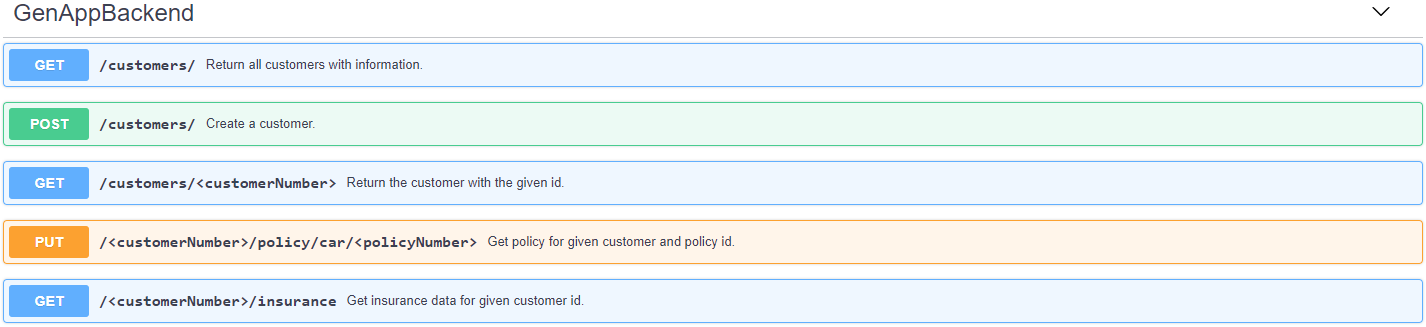
\includegraphics[scale=0.38]{images/kapitel_4/swagger_genappbackend.png}
  \caption{Übersicht des Backend-Interface}
  \label{fig:swagger_genappbackend}
\end{figure}

Für die Entwicklung des REST-Interfaces wird \path{Jersey}\footnote{https://github.com/jersey/jersey} genutzt. Mit Jersey
lässt sich ein Servlet-Endpunkt definieren, sodass der RESTful Web-Service in einem Servlet-Container wie dem WebSphere
Liberty läuft.

Bei Jersey werden über einzelne Funktionen \textit{Annotations} geschrieben, welche die zentrale Konfiguration des
Interfaces vornehmen. In Listing \ref{Beispiel eines REST-Endpunktes} auf Seite \pageref{Beispiel eines REST-Endpunktes}
ist eine Beispielimplementierung eines REST-Endpunktes zu sehen.

\begin{lstlisting}[language=java, caption=Beispiel eines REST-Endpunktes, label=Beispiel eines REST-Endpunktes]
    package de.larsprobst.rest;

    import javax.ws.rs.*;

    @Path("sayHello")
    public class MessageResource
    {
        @GET
        @Produces(MediaType.TEXT_PLAIN)
        public String message()
        {
            return "Hello";
        }
    }
\end{lstlisting}

In diesem kleinen Beispiel wird ein Endpunkt mit \path{/sayHello} erstellt, welcher über den Aufruf mit der HTTP-Methode
\path{GET} den Text \textit{Hello} zurück liefert.

In dieser Art werden alle benötigten Endpunkte für das REST-Interface definiert und mit Hilfe von Klassen werden
Objekte für Kundendaten und Policies erstellt.

Außerdem wird in einem Package die WOLA-Verbindung zur COBOL-Anwendung aufgebaut. Dies geschieht in diesem Beispiel über
die Klasse \path{GenAppJCAImpl.java}, welche alle Programmteile der COBOL-Anwendung kennt und diese nach Bedarf mit den
benötigten Parametern aufrufen kann.

Über die Klasse \path{GenAppCommarea.java} wird die Kommunikation zwischen Java- und COBOL-Anwendung definiert. Dort werden
die Java-Variablen auf die COBOL-Datentypen gemappt. Dies geschieht wie in Listing \ref{Java-Variable auf COBOL-Datentyp mappen}
auf Seite \pageref{Java-Variable auf COBOL-Datentyp mappen} beschrieben.

\begin{lstlisting}[language=java, caption=Java-Variable auf COBOL-Datentyp mappen, label=Java-Variable auf COBOL-Datentyp mappen]
    protected static final StringField CA_LAST_NAME = factory.getStringField(20);
\end{lstlisting}

In diesem Beispiel wird die Java-Variable \path{CA_LAST_NAME} auf einen COBOL-Datentyp gemappt, welcher insgesamt 20 Zeichen
besitzt. Die \path{factory} ist dabei vom Typ \path{CobolDatatypeFactory}, welche automatisch mit
\path{Java Batch Toolkit for z/OS (JZOS)} erstellt werden kann. Dabei analysiert das IBM Tool die genutzte COBOL-Anwendung
und erstellt die Klasse automatisiert.

Der Quelltext des Java-Wrappers ist im zugehörigen GitHub-Repository\footnote{https://github.com/Alienuser/GenAppBackend}
zu finden und kann dort heruntergeladen und genutzt werden.

\subsection{Erstellen des Web-Frontends}
Da nun die Schnittstellen des Java-Wrappers und auch die Rückgabewerte der Datenbank bekannt sind, kann das Web-Frontend
entwickelt werden. Dafür werden zuerst Use-Cases gesammelt, welche auf dem Frontend umgesetzt werden sollen. Anschließend
wird ein Mockup erstellt, welches das Design und die Anordnung darstellt.

Mit dem Web-Frontend soll es möglich sein, einerseits Daten aus der Datenbank über die COBOL-Anwendung mit Java-Wrapper
zu laden, als auch über den DB2 REST Service.

Außerdem soll ein weiterer Bereich entstehen, in dem Daten aus einem Watson-Service gelesen werden können. Dabei handelt
es sich um einen Kundenwert des Nutzers, welcher anhand von Beispieldaten berechnet wird.

Die Daten sollen nicht nur einmalig aus der Datenbank geholt werden, sondern via \textit{polling} alle 15 Sekunden. Die
Idee dahinter ist, dass Daten in der Datenbank abgeändert werden können und sich diese nach maximal 14 Sekunden auch im
Frontend ändern. Da CICS-Regionen zur Zeit kein \textit{Web-Socket} unterstützen, muss dies via \textit{polling} gelöst
werden.

Da das Frontend auch in den Smartphone-Apps angezeigt werden soll ist es wichtig, dass es sich der Größe des Bildschirmes
anpasst, mit dem es angezeigt wird. Allgemein ist es wichtig, eine Mobile-First- oder Responsive-Webseite zu erstellen.

Das entstandene Mockup kann in Abbildung \ref{fig:mockup_website} auf Seite \pageref{fig:mockup_website} angesehen werden.
Dabei fällt auf, dass es neben den Boxen für die Informationen auch eine Navigationsleiste mit zwei Menüpunkten gibt.

\begin{figure}[h]
 \centering
   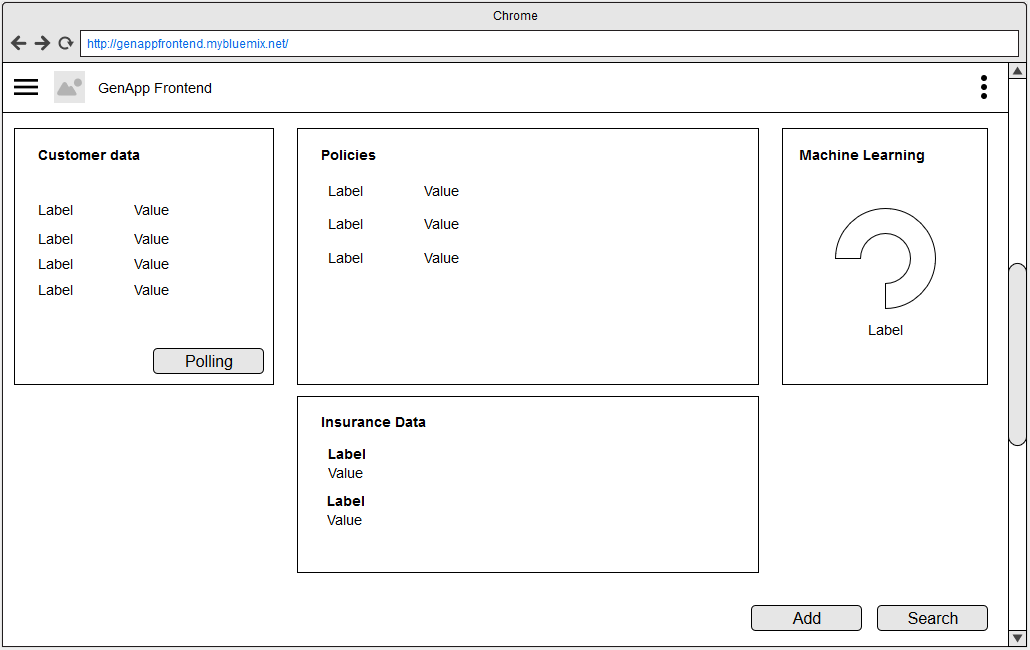
\includegraphics[scale=0.5]{images/kapitel_4/mockup_website.png}
 \caption{Mockup des Web-Frontends}
 \label{fig:mockup_website}
\end{figure}

Der linke Menüpunkt (auch \textit{Burgermenü} genannt), öffnet das seitliche Navigationsmenü. Dort gibt es allerdings nur einen
Eintrag, welcher auch standardmäßig geöffnet und ausgewählt ist. Die Idee dabei ist, dass das Frontend in Zukunft
weiterentwickelt werden kann und dann mehrere Menüpunkte benötigt werden, welche alle in diesem seitlichen Menü angezeigt
werden können.

Das rechte Menü mit den drei übereinanderstehenden Punkten symbolisiert ein Kontextmenü, welches ein Dropdown öffnet. In
diesem gibt es zwei Menüeinträge. Einen \path{Settings} und einen \path{Info} Eintrag. Ersterer kann die verwendete URL
des Secure Gateways überschreiben, damit für Demonstrationszwecke andere Endpunkte genutzt werden können.

Zweiterer öffnet ein modales Fenster, welches Informationen über die vorliegende App
anzeigt, einen Link zum GitHub-Repository beinhaltet und Kontaktmöglichkeiten mit dem Autoren zur Verfügung stellt.

Am unteren rechten Bildschirmrand wird es zwei Buttons geben. Einer wird eine Suche nach einer Kundennummer ermöglichen.
Der Andere öffnet ein modales Fenster, mit welchem ein neuer Benutzer in die Datenbank eingetragen werden kann.

Nach jeder Suche oder der Anzeige von Daten soll am unteren linken Bildschirmrand eine kleine Informationsbox erscheinen,
welche Informationen anzeigt. So zum Beispiel das erfolgreiche Auffinden eines Nutzers oder wenn Probleme aufgetreten sind.

Abbildung \ref{fig:frontend_browser} auf Seite \pageref{fig:frontend_browser} zeigt das fertig entwickelte Web-Frontend,
wie es in einem Desktopbrowser angezeigt wird.

\begin{figure}[h]
 \centering
   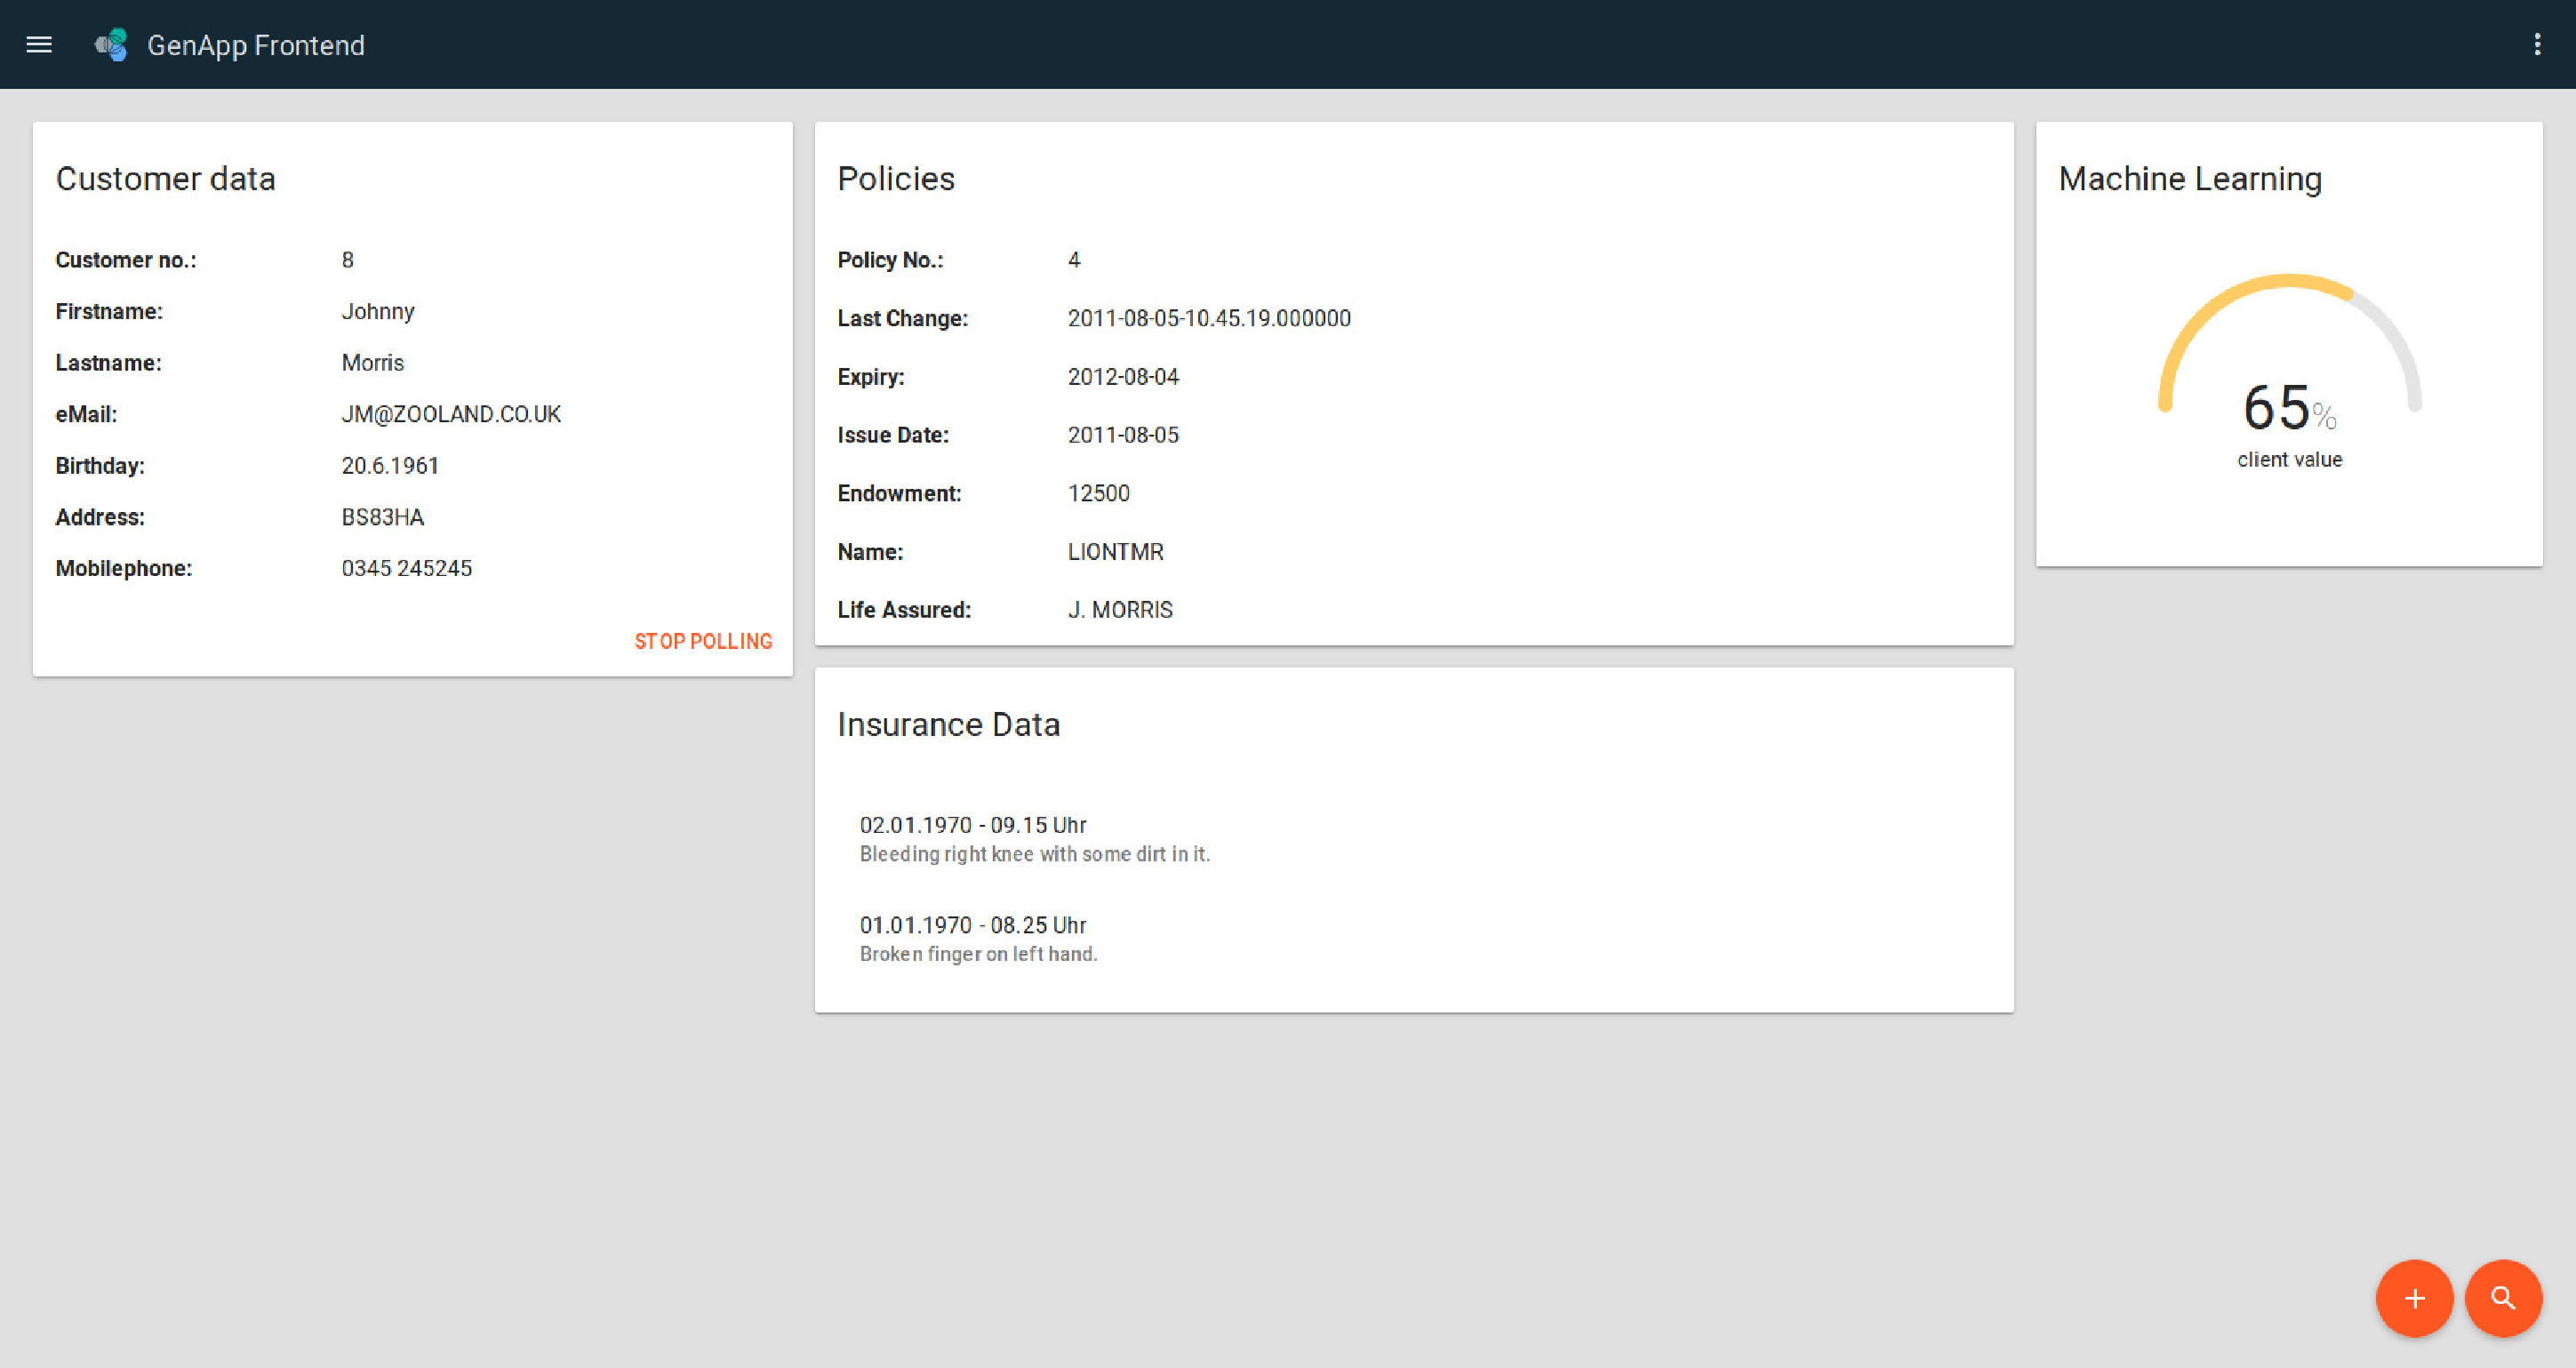
\includegraphics[scale=0.29]{images/kapitel_4/frontend_browser.pdf}
 \caption{Web-Frontend im Browser}
 \label{fig:frontend_browser}
\end{figure}

In Abbildung \ref{fig:frontend_smartphone} auf Seite \pageref{fig:frontend_smartphone} ist das Web-Frontend mit einem
emulierten Smartphone zu sehen. Es handelt sich dabei um eine Auflösung von 360x640 Pixel. In dieser Abbildung
ist ersichtlich, wie das Frontend sich an die Größe des Bildschirms anpasst. In der Größe eines Smartphones würde das
seitliche Menü auch den kompletten sichtbaren Bereich der Webseite überdecken.

Auch die Größe der modalen Fenster ist in der Größe eines Smartphones breiter, damit Daten einfacher eingegeben werden
können.

\begin{figure}[h]
 \centering
   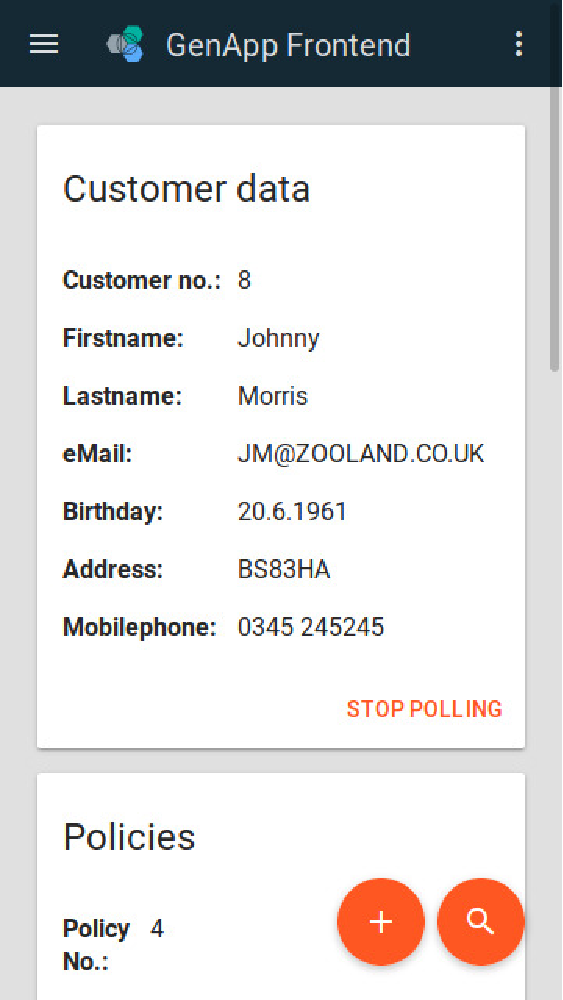
\includegraphics[scale=0.64]{images/kapitel_4/frontend_smartphone.pdf}
 \caption{Web-Frontend im Smartphone}
 \label{fig:frontend_smartphone}
\end{figure}

Die beiden REST-Interfaces des Backends, der Java-Wrapper und der DB2 REST Service, werden in der Umsetzung mit
Angular-Factories angesprochen. Das hat den Vorteil, dass für jedes Backend eine Factory geschrieben wird, die jedem
Controller zur Verfügung gestellt werden kann.

Da nur eine Seite exisitert, wird auch nur ein Angular-Controller benötigt. Dieser kümmert sich um die Übermittlung der
Daten an die \textit{View}, nachdem ein Polling oder eine Suche gestartet wird.

Mit der Cloud Foundry CLI und dem Befehl \path{push} kann das Web-Frontend an Bluemix übertragen und mit der in Kapitel
\ref{subsec:runtime_hinzufügen} auf Seite \pageref{subsec:runtime_hinzufügen} erstellte Cloud Foundry Runtime zur Verfügung
gestellt werden.

Der komplette Quelltext des Frontends ist im zugehörigen GitHub-Repository\footnote{https://github.com/Alienuser/GenAppFrontend}
zu finden. Dieser kann bequem geklont und anschließend in der eigenen Cloud Foundry Runtime zur Verfügung gestellt
werden.

\subsection{Erstellen der Smartphone App}
Da das Web-Frontend nun fertig gestellt ist und über eine Domain mit einem Webbrowser aufgerufen werden kann, können die
Smartphone-Apps erstellt werden, welche das Web-Frontend in einem WebView-Layout laden und darstellen.

Dabei wird dem Layout die Domain übergeben und das Layout kümmert sich selbstständig um die Darstellung der Webseite und
die Interaktion damit.

Da der Aufbau einer Smartphone-App für die verschiedenen Betriebsysteme stark abweicht, wird in den folgenden beiden
Kapiteln die Spezifika der Android- und der iOS-App aufgezeigt. Dabei werden Projekte für die jeweiligen Betriebssysteme
erstellt und die Anwendung entwickelt.

\subsubsection{Android}
Zur Erstellung einer Android-App wird die \path{Android Studio IDE} benötigt. Diese kann kostenlos auf der
Developer-Seite\footnote{https://developer.android.com/studio/index.html} von Google heruntergeladen werden und steht für
Windows, Linux und MacOS zur Verfügung. Android Studio basiert auf der Community Version von
IntelliJ\footnote{https://www.jetbrains.com/idea}.

Für die Verwendung von Android Studio wird eine Installierte \textit{Java-JRE} und das \textit{Java-JDK} benötigt. Die
Java-JRE wird für das Ausführen der IDE genutzt. Das Java-JDK zum Bauen des Quellcodes auf dem Entwicklersystem. Es wird
empfohlen, jeweils die aktuellste Version zu nutzen. Dies ist zur Zeit jeweils Version 8.

Nach der Installation und dem ersten Start von Android Studio muss ein \textit{Android-SDK} sowie ein Emulator heruntergeladen
werden. Dabei werden jeweils die neuesten Versionen ausgewählt. Für das SDK bedeutet das \path{26.0.2} und für den Emulator
\path{Android O} bzw. \path{Android 8}. Mit dem Emulator kann die App später getestet werden. Dabei handelt es sich um ein
vollwertiges Betriebssystem mit allen Möglichkeiten.

Im nächsten Schritt wird ein neues Android-Projekt angelegt. Dazu wird als Name \path{GenAppAndroid} gewählt und ein leeres
Projekt selektiert.

Die Android-App muss im Ordner \path{/res/layout} ein Layout besitzen, welches als Root-Element ein \path{CoordinatorLayout}
besitzt und als Kind-Element ein {WebView} Layout. Diesem wird eine \textit{ID} zugeteilt, damit es aus dem Java-Teil
eindeutlig identifiziert werden kann.

Im Java-Teil wird neben einer \textit{Splashscreen}- noch eine \textit{Main}-Activity hinzugefügt. Erstere soll nach dem
Start der Anwendung das Logo mit entsprechendem Hintergrund anzeigen und erst auf die Main-Activity wechseln, wenn die
Webseite geladen ist.

Die Main-Activity besitzt als unveränderliche Variable die URL des Web-Frontends und konfiguriert in der
\path{onCreate}-Methode das WebView-Layout, damit es JavaScript akzeptiert. Anschließend wird die Webseite im Layout
angezeigt.

Das WebView-Layout, welches von \path{Android-Webkit} erbt, kümmert sich anschließend um die korrekte Darstellung der
Webseite und die Interaktion des Nutzers mit dieser. Mit dem Überschreiben von Funktionen im \path{WebViewClient} kann
das Verhalten des Layouts angepasst werden. So kann zum Beispiel Einfluss auf den Titel oder sogar HTML-Elemente
genommen werden.

In den \path{/res/values} und \path{/res/values-21}-Ordnern werden Farben und Styles definiert. In letzterem lediglich
Styles, die ab Android SDK-Version 21 genutzt werden sollen.

Die Ordner- und Dateistruktur kann in der Abbildung \ref{fig:androidstudio_folder} auf Seite \pageref{fig:androidstudio_folder}
eingesehen werden.

\begin{figure}[h]
 \centering
   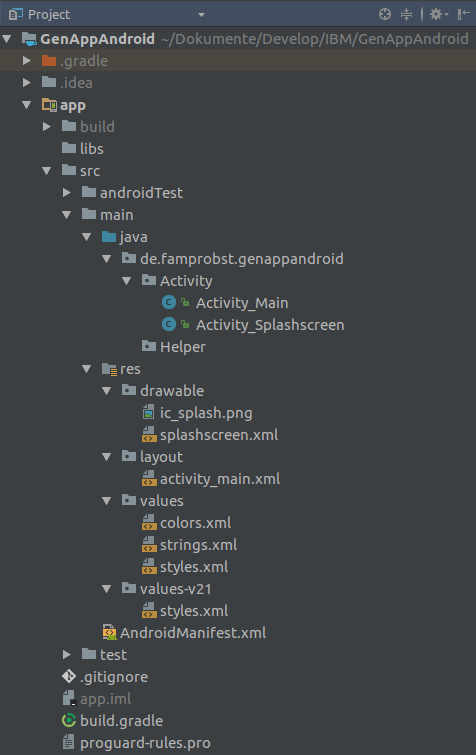
\includegraphics[scale=0.4]{images/kapitel_4/androidstudio_folder.png}
 \caption{Ordner und Dateien in Android Studio}
 \label{fig:androidstudio_folder}
\end{figure}

Im Ordner \path{/res/drawable} ist das Logo der Anwendung (das Bluemix Logo) und auch die Konfiguration des
Splashscreen-Hintergrundes hinterlegt.

Die \path{Manifest.xml}-Datei entählt Informationen und Konfigurationen der Android-App. Zum Beispiel wird in dieser Datei
angegeben, welche Activity beim Start der Anwendung geöffnet werden soll oder welche Styles genutzt werden sollen. Mehr
Informationen dazu gibt es auf den Developer-Seiten\footnote{https://developer.android.com/guide/topics/manifest/manifest-intro.html}
von Android.

In der Abbildung \ref{fig:frontend_smartphone_android} auf Seite \pageref{fig:frontend_smartphone_android} ist die fertig
entwickelte Android-App auf einem Smartphone-Emulator zu sehen.

\begin{figure}[h]
 \centering
   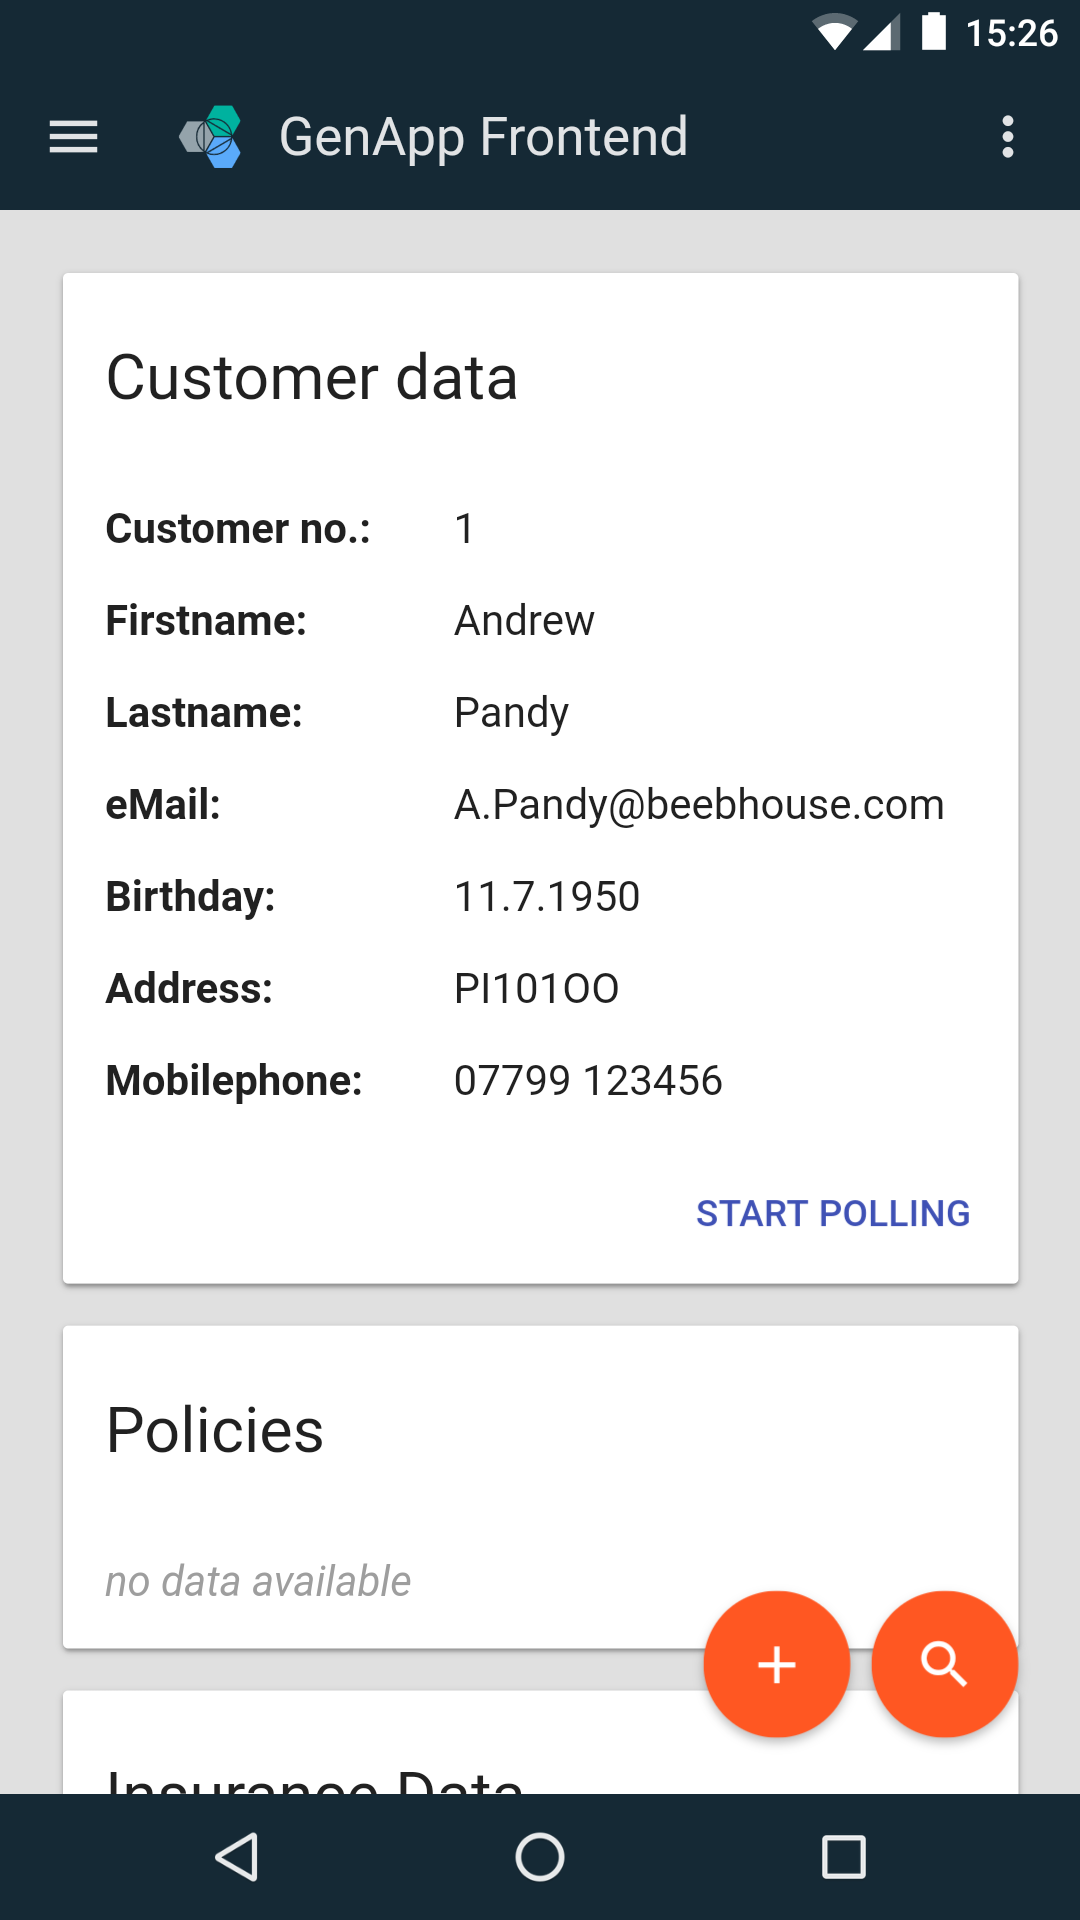
\includegraphics[scale=0.19]{images/kapitel_4/frontend_smartphone_android.png}
 \caption{Android-App im Smartphone-Emulator}
 \label{fig:frontend_smartphone_android}
\end{figure}

In dieser Abbildung ist sichtbar, dass die Android-Styles Einfluss auf die Darstellung der Menüpunkte (am unteren Rand)
und die Farbe des Toolbar nehmen kann. Beide werden in der selben Farbe wie der Header im Web-Frontend dargestellt.

In der Abbildung \ref{fig:frontend_tablet_android} auf Seite \pageref{fig:frontend_tablet_android} wird die Anwendung in
einem Tablet-Emulator gezeigt. Im Vergleich der beiden Screenshots ist gut zu sehen, dass sich das Frontend den Gegebenheiten
wie zum Beispiel Bildschirmgröße gut anpasst.

\begin{figure}[h]
 \centering
   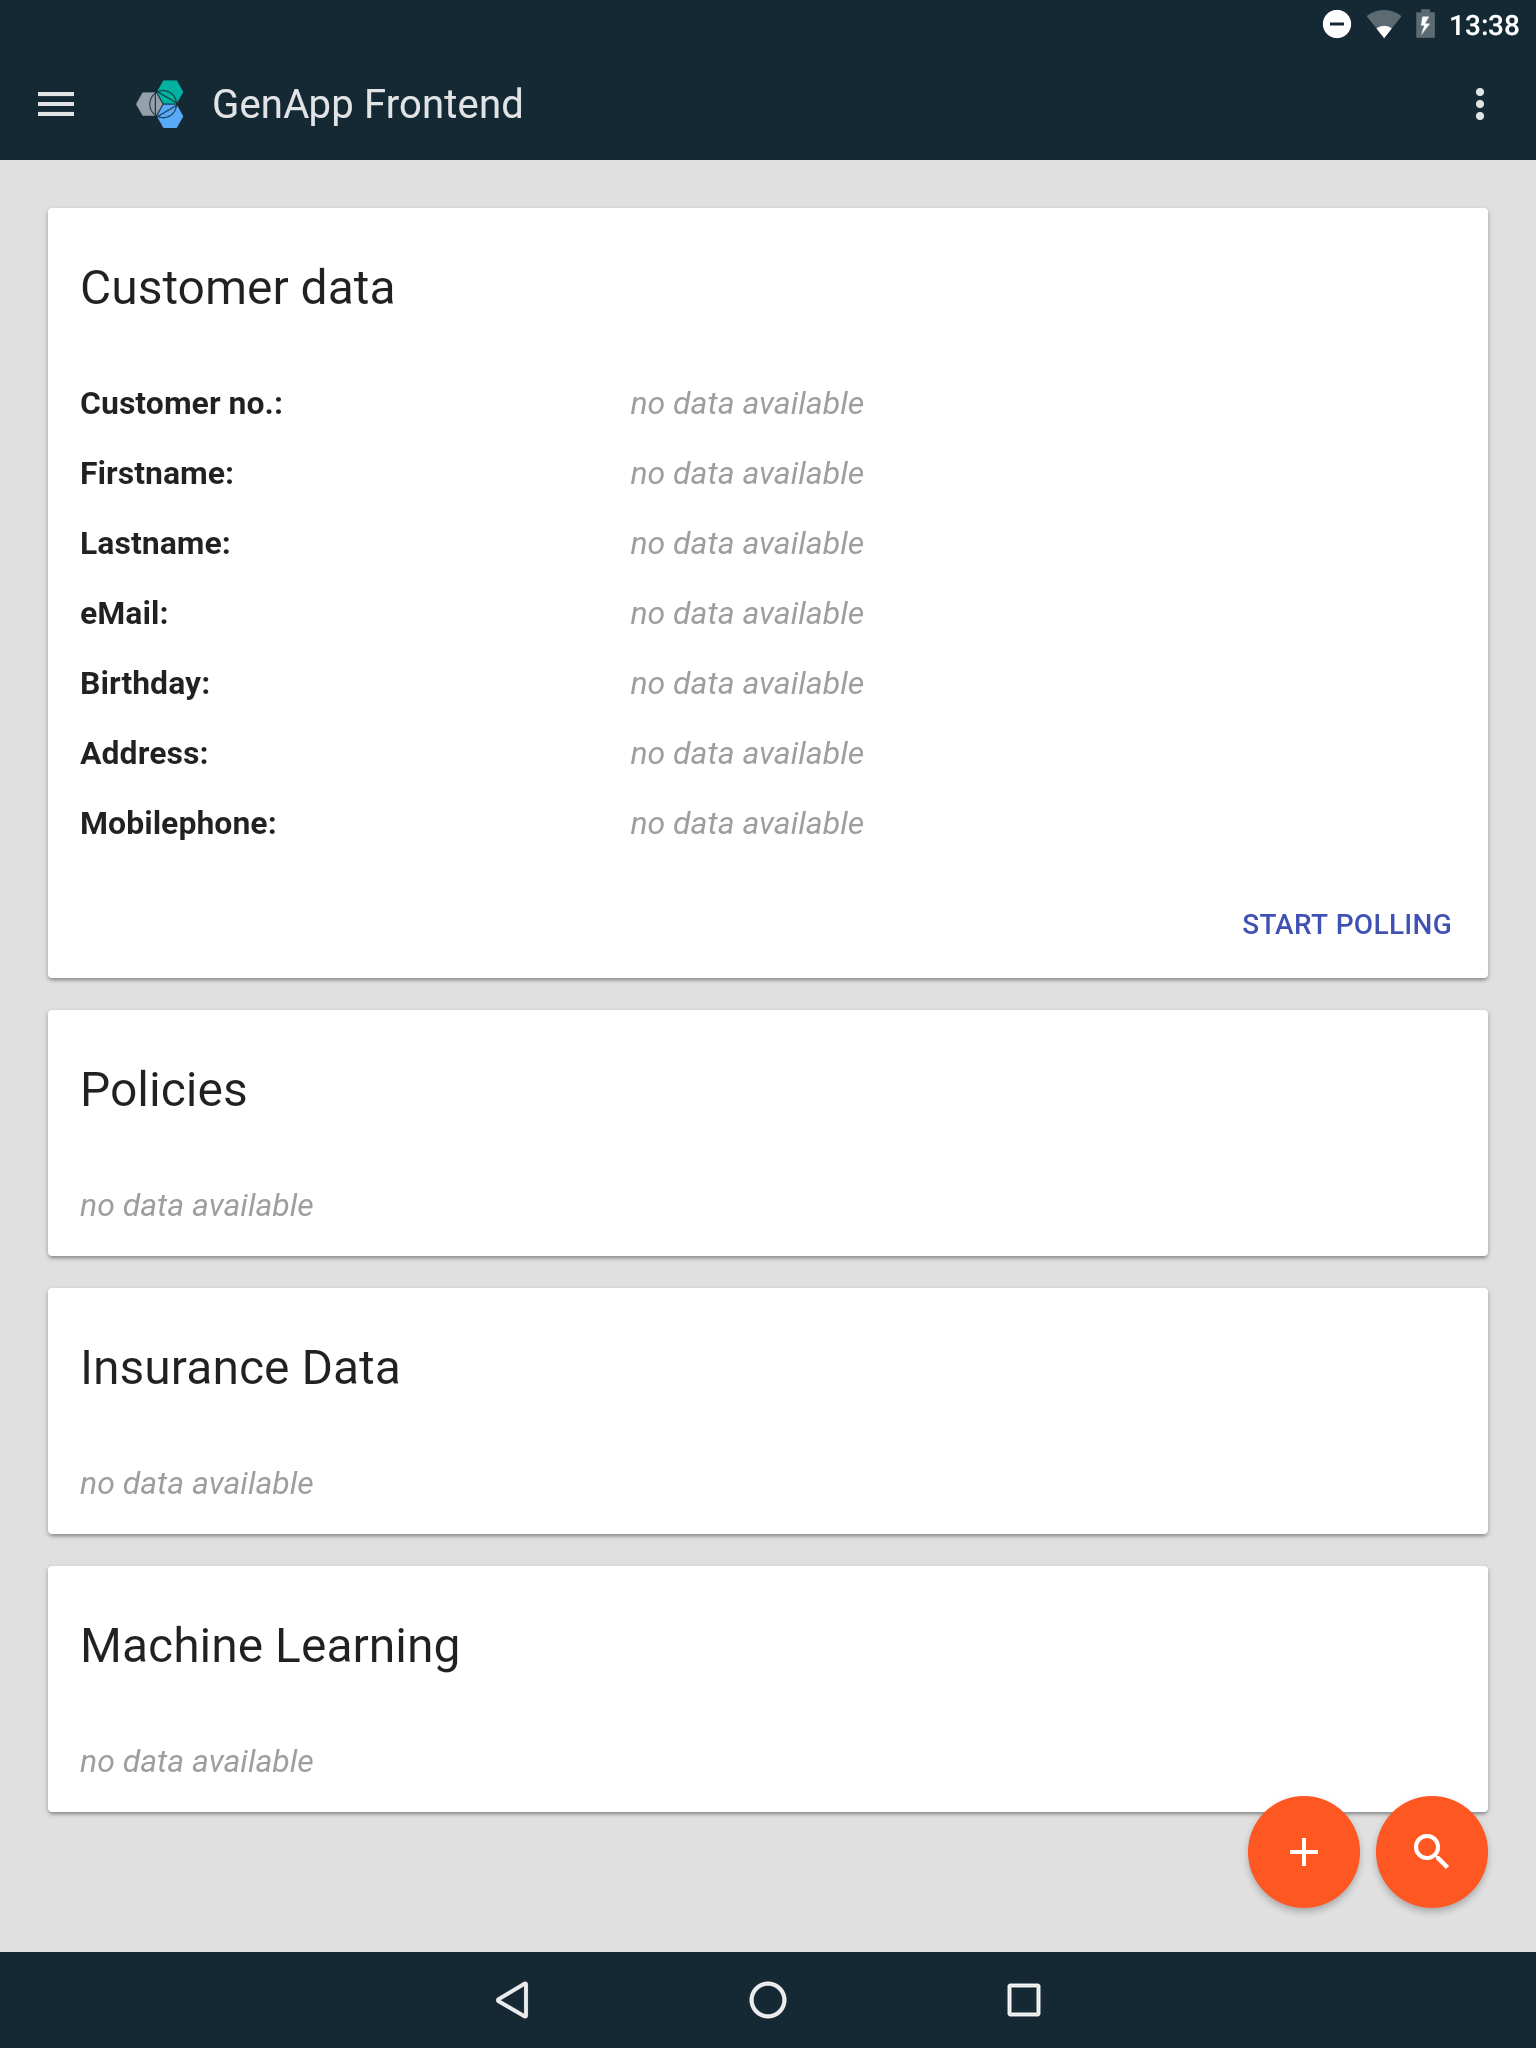
\includegraphics[scale=0.18]{images/kapitel_4/frontend_tablet_android.png}
 \caption{Android-App im Tablet-Emulator}
 \label{fig:frontend_tablet_android}
\end{figure}

Der Quelltext der Android-App kann im GitHub-Repository\footnote{https://github.com/Alienuser/GenAppAndroid} eingesehen
werden.

Es ist möglich das GitHub-Projekt direkt in Android Studio zu klonen und als Projekt zu nutzen. Dazu muss beim Start von
Android Studio \path{Check out project from version control} ausgewählt werden, worauf die GitHub-URL eingegeben werden
muss.

Das Projekt wird nun automatisch angelegt und der benötigte Gradle-Wrapper heruntergeladen. Anschließend wird das Projekt
direkt gebaut und die benötigten Abhängigkeiten heruntergeladen. Anschließend kann die App in einem beliebigen Emulator
getestet werden.

Die Android-App ist nun fertig entwickelt und kann exportiert werden. Dazu wird eine \textit{Signing}-Datei erstellt
mit welcher es möglich ist, die Anwendung auch in den Play-Store zu laden. Alternativ kann die exportierte
\textit{Android Package}-Datei (kurz APK) auch auf echten Geräten installiert werden.

\clearpage
\newpage

\subsubsection{iOS}
Um eine App für iOS Geräte zu entwickeln, wird die kostenlose IDE \path{XCode} benötigt. Diese steht lediglich MacOS-Geräten
zur Verfügung und kann auf der Developer-Seite\footnote{https://developer.apple.com/xcode} von Apple heruntergeladen werden.

Somit ist das Schreiben, Kompilieren und Testen einer iOS-App unter XCode nur unter MacOS möglich, was eine große
Einschränkung darstellt.

Nach der Installation wird in XCode anschließend ein neues Projekt angelegt. Die Art des Projektes ist \path{SingleViewApp}
und der Name ist zum Beispiel \path{GenAppiOS}. In Abbildung \ref{fig:xcode_overview} auf Seite \pageref{fig:xcode_overview}
ist das erstellte Projekt in XCode zu sehen. Der Emulatoren und die verschiedenen SDKs werden automatisch installiert.

\begin{figure}[h]
 \centering
   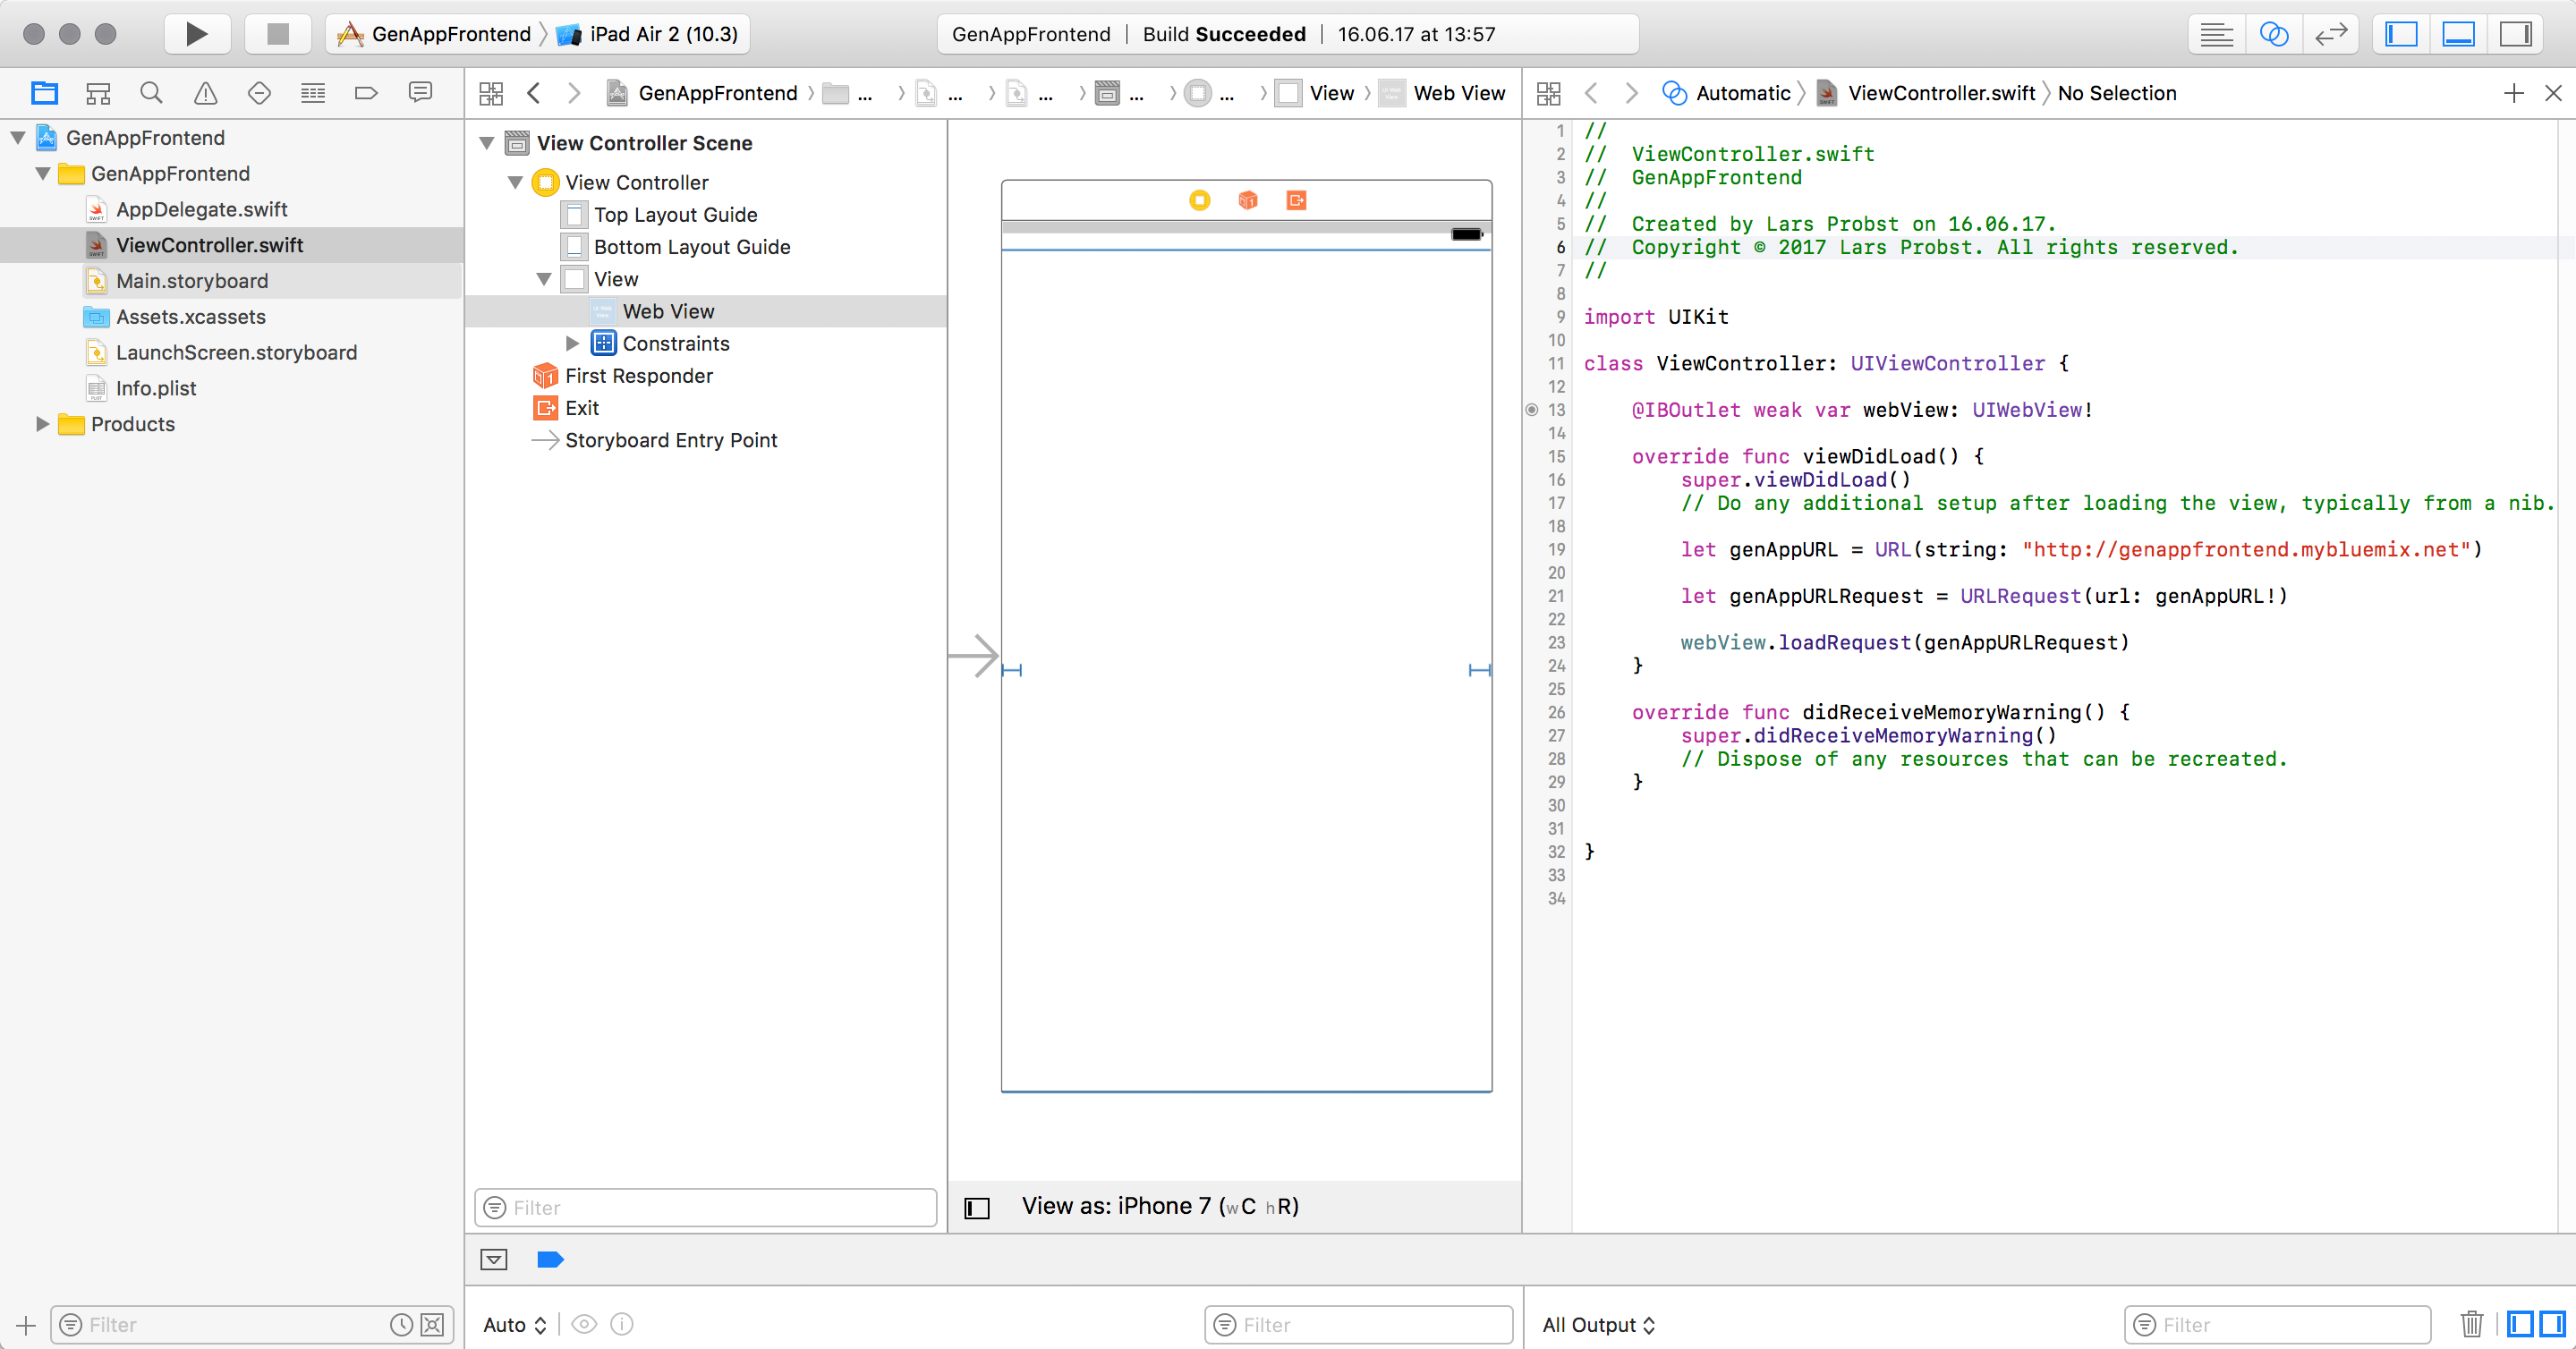
\includegraphics[scale=0.26]{images/kapitel_4/xcode_overview.png}
 \caption{Übersicht von XCode}
 \label{fig:xcode_overview}
\end{figure}

Bei den beiden \path{.swift}-Dateien handelt es sich um die ausführbaren Klassen innerhalb der Anwendung. Ihn ihnen wird
die Logik entwickelt.

Dabei wird in der \path{ViewController}-Datei die genutzte View konfiguriert und, wie in der Abbildung zu sehen, zum
Beispiel dem WebView-Layout die URL des Web-Frontends übergeben.

In der \path{AppDelegate}-Datei wird der Lifecycle der Anwendung definiert. So wird dort festgelegt, dass der genutzte
Controller das \path{LaunchScreen}-Storyboard zugeteilt bekommt.

Die \path{.storyboard}-Dateien sind für die Darstellung der einzelnen Seiten und Menüs zuständig. Davon wird in diesem
Projekt nur eine benötigt, welche das Web-Frontend darstellen kann.

Als Letztes wird die \path{.plist}-Datei für die Konfiguration der Anwendung benötigt. Sie ist ähnlich der
Android-Manifest-Datei.

In Abbilung \ref{fig:xcode_folder} auf Seite \pageref{fig:xcode_folder} ist eine Übersicht der Ordnerstruktur in XCode
abgebildet. Dort sind alle genutzten Dateien sichtbar.

\begin{figure}[h]
 \centering
   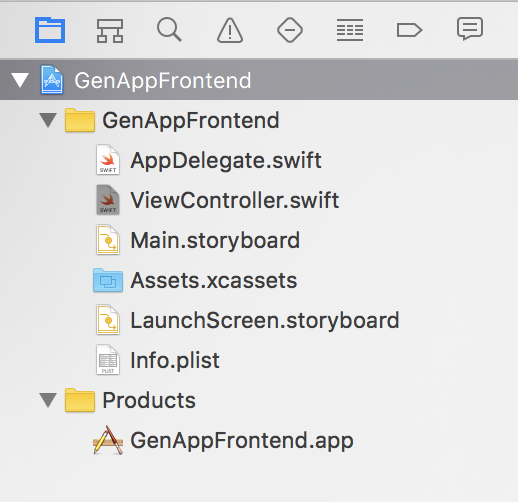
\includegraphics[scale=1]{images/kapitel_4/xcode_folder.png}
 \caption{Ordner und Dateien in XCode}
 \label{fig:xcode_folder}
\end{figure}

Die Plist-Datei (Property List Files) beinhaltet die Konfiguration der Anwendung. So wird hier zum Beispiel eingestellt,
ab welcher Version die Anwendung zur Verfügung stehen soll und ob es zum Beispiel Einschränkungen in der Ausrichtung der
App geben soll. Außerdem wird der Name der Anwendung und das verwendete Icon definiert.

Anschließend wird im Storyboard, der View, ein WebView-Layout angelegt. Dieses wird mit der Programmiersprache Swift dann
angesprochen und konfiguriert. Ähnlich der Android-App werden Informationen wie Domain oder Anzeigegröße übergeben und das
Layout kümmert sich eigenständig um das Laden, das Darstellen und die Interaktion mit dem Nutzer der Webseite.

Nach einem Klick auf \path{Run} (kleiner schwarzer Play-Button) in XCode, kann der Emulator ausgewählt werden, mit welchem
die Anwendung gestartet werden soll. In der Abbilung \ref{fig:frontend_smartphone_ios} auf Seite
\pageref{fig:frontend_smartphone_ios} ist die Anwendung im Smartphone Emulator mit der neuesten iOS Version zu sehen.

\begin{figure}[h]
 \centering
   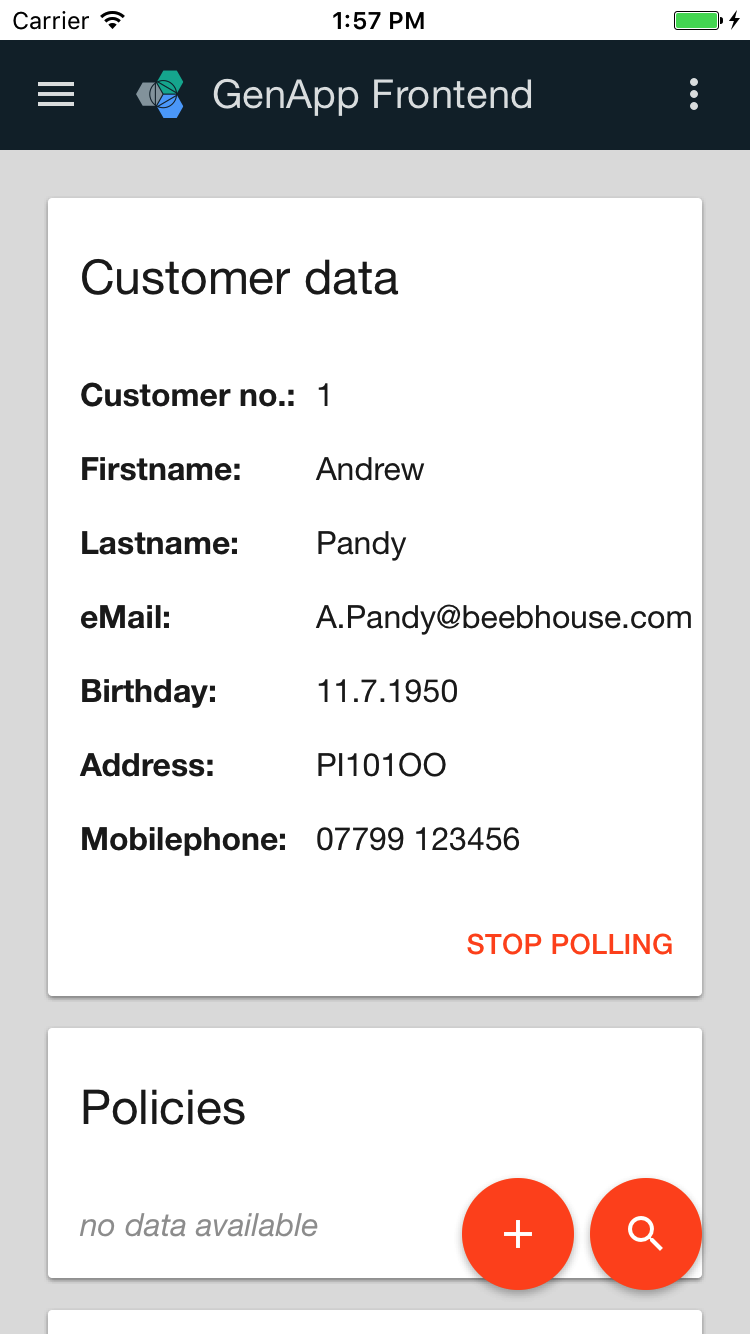
\includegraphics[scale=0.28]{images/kapitel_4/frontend_smartphone_ios.png}
 \caption{iOS-App im Smartphone-Emulator}
 \label{fig:frontend_smartphone_ios}
\end{figure}

Die Abbildung \ref{fig:frontend_tablet_ios} auf Seite \pageref{fig:frontend_tablet_ios} hingegen zeigt die Anwendung in
einem Tablet-Emulator mit ebenfalls der neuesten iOS Version.

Auch in diesen beiden Version zeigt sich, dass sich das Web-Frontend gut an die Displaygrößen anpasst. Dies ist gewünscht,
da sonst eine Interaktion mit der Webseite nicht bzw. schwer möglich ist.

Leider ist es unter iOS nicht möglich die Farbe der Titleleiste einzustellen, sodass sie hier einfach weiß, wie vom System
definiert, bleibt. Ansonsten würde sich die Titelleiste besser in das Gesamtlayout eingliedern.

\begin{figure}[h]
 \centering
   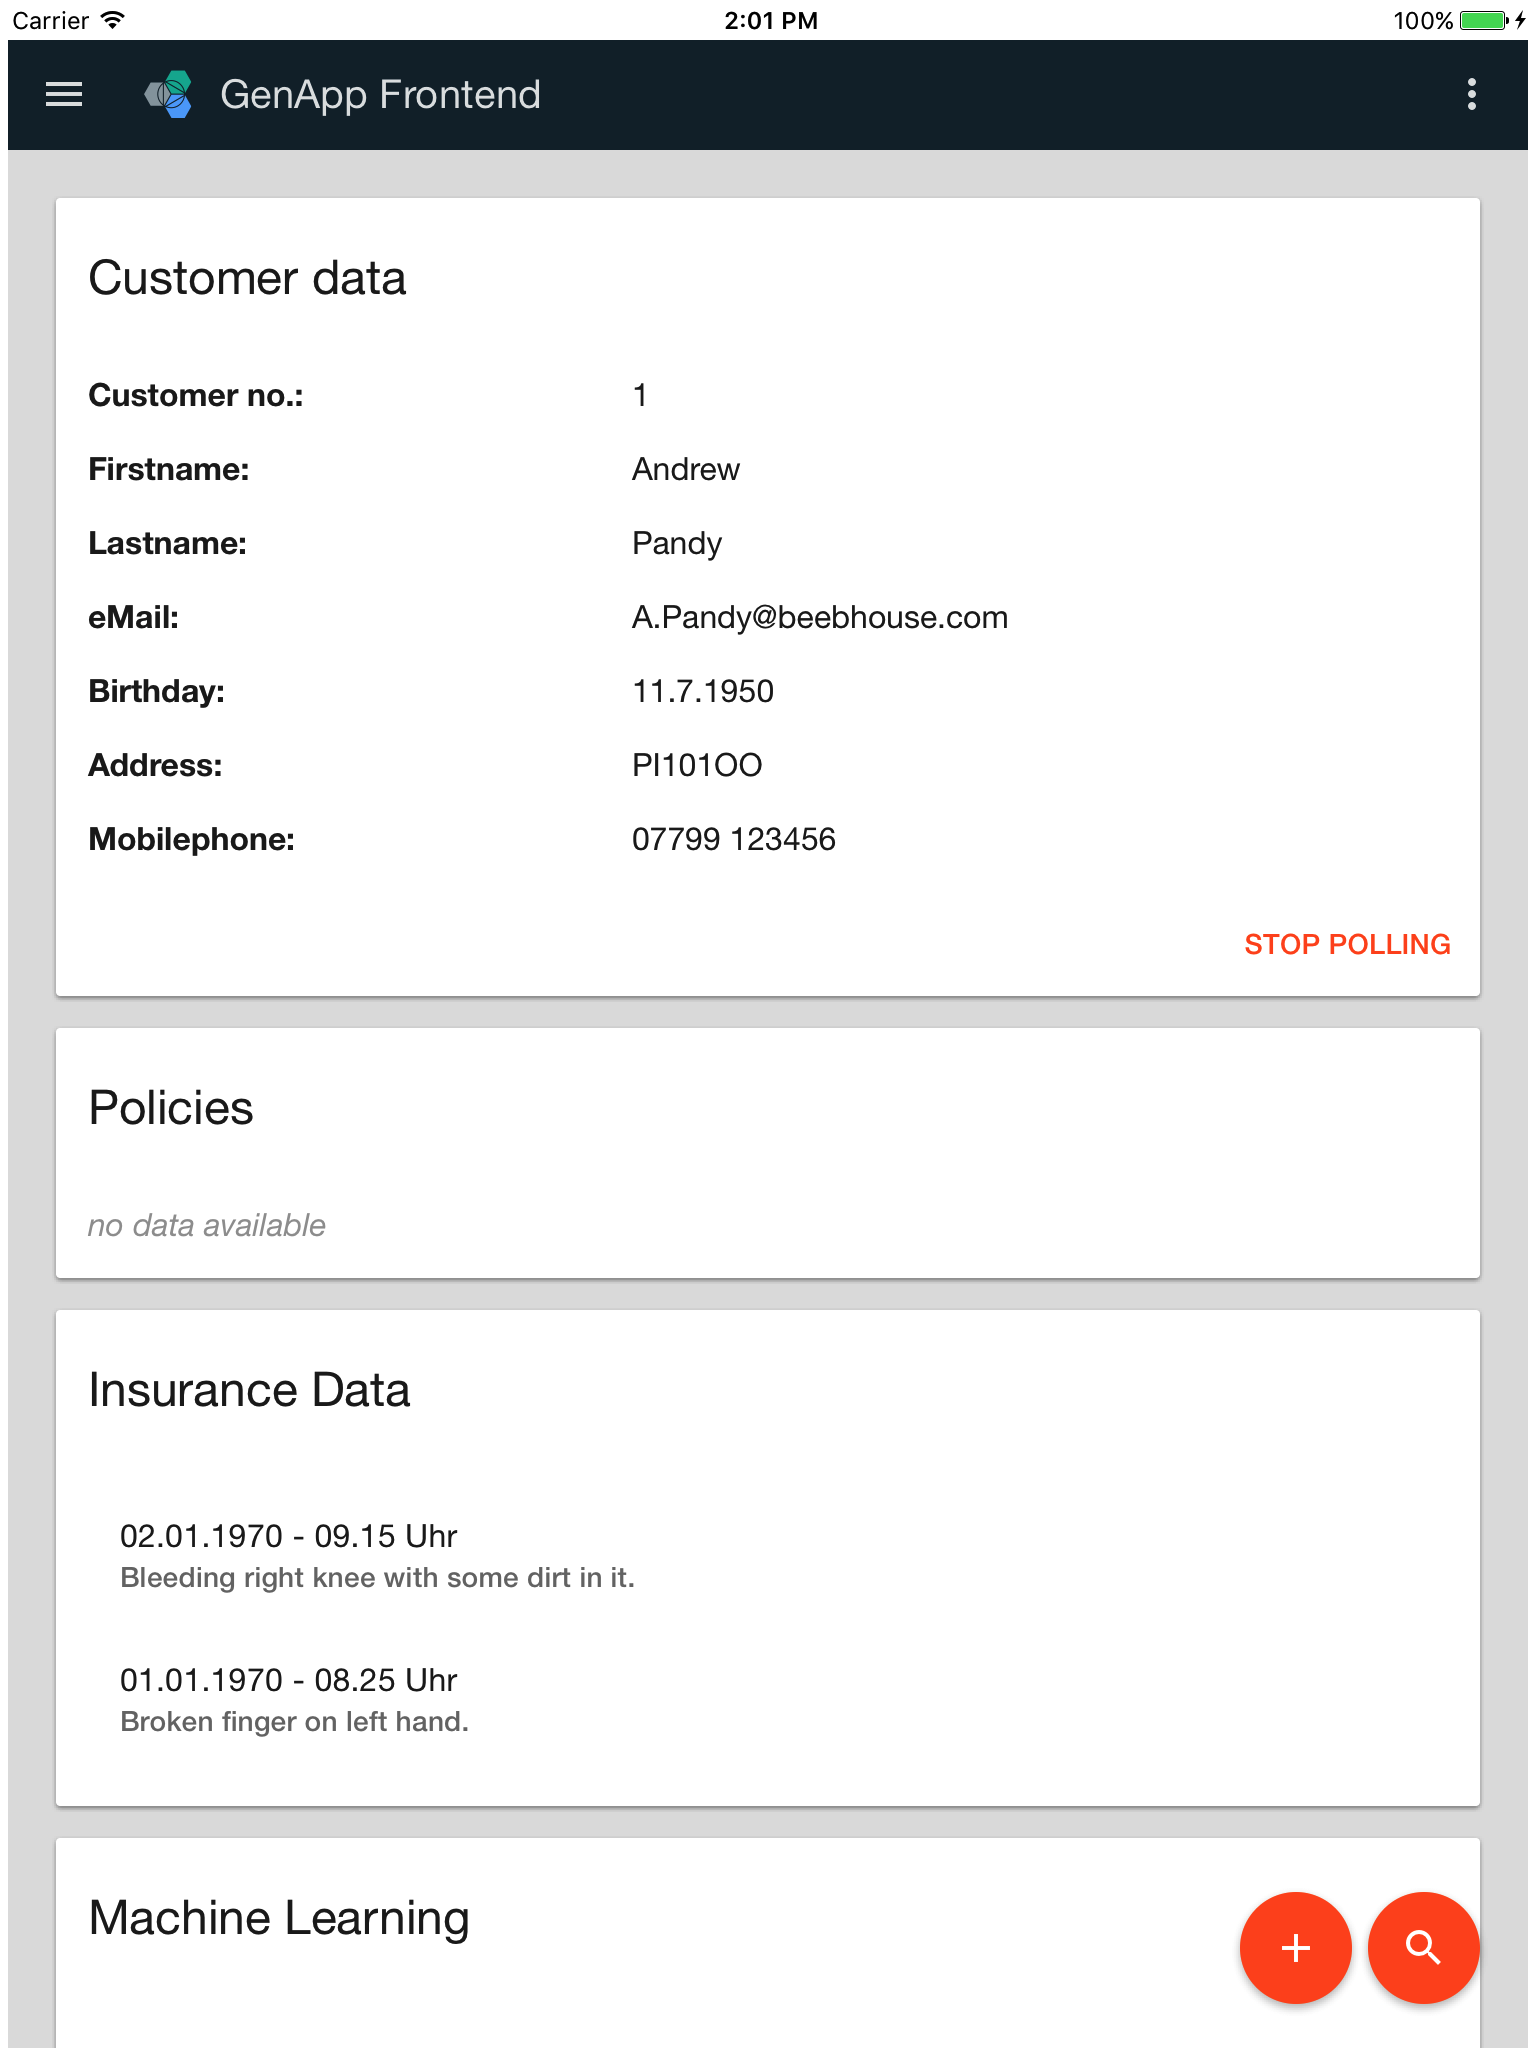
\includegraphics[scale=0.2]{images/kapitel_4/frontend_tablet_ios.png}
 \caption{iOS-App im Tablet-Emulator}
 \label{fig:frontend_tablet_ios}
\end{figure}

Die iOS-App kann nun exportiert und nach Bedarf auf echten Geräten installiert werden. Alternativ ist es auch möglich
die Version in den App-Store zu laden.